% Document generat per llibre/llibre.py a partir de docs/nombres-reals/.
% No l'editis a mà: torna'l a generar.
\documentclass[11pt,a4paper,twoside,openright]{book}
\usepackage{apunts}
\hypersetup{pdftitle={Matemàtiques I. Tema 1: Nombres reals},pdfauthor={Jordi Irazuzta i Ignasi Irazuzta},pdflang={ca}}
\begin{document}
\frontmatter
\portada{1}{Nombres reals}{1r de Batxillerat}
\cleardoublepage
\tableofcontents
\mainmatter
\setcounter{chapter}{0}
% Contingut generat per llibre/llibre.py a partir de docs/nombres-reals/.
% No l'editis a mà: torna'l a generar.

\chapter{Nombres reals}

Fixa't que els nombres reals ja els fas servir cada dia: preus, mesures, percentatges, distàncies... En aquest tema hi posarem ordre. Repassarem d'on surten (naturals, enters, racionals i irracionals) i aprendrem a situar-los i comparar-los a la recta real, a treballar amb intervals i valor absolut, i a manejar amb soltesa potències, arrels i logaritmes.

Recorda que aquestes eines et serviran durant tot el curs, així que val la pena dominar-les bé des del principi.

\section{El conjunt dels nombres reals}

Segur que ja coneixes molts conjunts de nombres dels cursos anteriors. Repassem-los ara amb una mica més de rigor, per veure com s'encaixen els uns dins dels altres.

Comencem pel conjunt més senzill: els \textbf{nombres naturals}, els que fem servir per comptar els elements d'un conjunt finit:

\[
\mathbb{N} = \{0, 1, 2, 3, 4, \dots\}
\]

\begin{nota}{Notació: conjunts finits i infinits numerables}
Un conjunt finit o infinit numerable s'escriu entre claus, amb els elements separats per comes: $\{e_1, e_2, e_3, \dots\}$. Quan el conjunt és infinit, els punts suspensius ($\dots$) indiquen que el patró continua indefinidament sense acabar-se mai.
\end{nota}

Fixa't que el $0$ és l'\textbf{element neutre} de la suma i l'$1$ ho és del producte: sumar-hi $0$ o multiplicar-hi per $1$ no altera el nombre original. Per exemple, amb el $4$:

\[
4 + 0 = 0 + 4 = 4 \qquad\qquad 4 \cdot 1 = 1 \cdot 4 = 4
\]

Podem ampliar el conjunt dels naturals afegint, per a cada nombre, el seu \textbf{oposat}: el nombre que, sumat a l'original, dona $0$. El notem amb un $-$ al davant:

\[
5 + (-5) = 0
\]

Fixa't que l'oposat de l'oposat torna a ser el nombre original:

\[
-(-5) = 5
\]

Si afegim als naturals tots els seus oposats, obtenim els \textbf{nombres enters}:

\[
\mathbb{Z} = \{\dots, -3, -2, -1, 0, 1, 2, 3, \dots\}
\]

Un cop tenim els enters, la resta ja no és cap operació nova: no és més que sumar l'oposat.

\[
8 - 3 = 8 + (-3) = 5
\]

I ara, gràcies als enters, també podem restar un nombre gran d'un de més petit, cosa que amb només naturals no podíem fer:

\[
3 - 8 = 3 + (-8) = -5
\]

Tot nombre, a més, es pot escriure en forma decimal: part entera i part decimal separades per una coma. Per exemple:

\[
-6 = -6{,}0 \qquad 1{,}56 \qquad 1{,}\overline{3} \qquad \pi = 3{,}141592\dots
\]

Aquesta representació decimal ens permet separar els nombres en dos grans grups: els \textbf{racionals} ($\mathbb{Q}$), que es poden escriure com una fracció, i els \textbf{irracionals} ($\mathbb{R}\setminus\mathbb{Q}$), que no:

\[
x \in \mathbb{Q} \;\;\Leftrightarrow\;\; \exists\, m,n \in \mathbb{Z},\; n \neq 0 \;\; \text{tals que } x=\frac{m}{n}
\]

\begin{nota}{Pertinença}
Quan un element pertany a un conjunt fem servir el símbol $\in$; si no hi pertany, $\notin$.

Exemple: $-3 \in \mathbb{Z}$, però $-3 \notin \mathbb{N}$.
\end{nota}

\begin{nota}{Implica i equival}
$\Rightarrow$ es llegeix "aleshores" (implica). $\Leftrightarrow$ es llegeix "equival" (si i només si).

Exemple: $x \in \mathbb{N} \Rightarrow x \in \mathbb{Z}$ — si $x$ és natural, també és enter.
\end{nota}

Dins dels racionals no enters, en trobem de dos tipus: els \textbf{exactes} (part decimal amb un nombre finit de xifres) i els \textbf{periòdics} (la part decimal es repeteix indefinidament seguint un patró, pur o mixt).

\begin{nota}{Quantificadors}
$\forall$ es llegeix "per a tot". $\exists$ es llegeix "existeix" o "hi ha".

Exemple: $\forall n \in \mathbb{N},\; n+1 \in \mathbb{N}$ — per a tot natural $n$, $n+1$ també ho és.
\end{nota}

Aquest esquema resumeix tota la divisió que acabem de fer:

\begin{center}
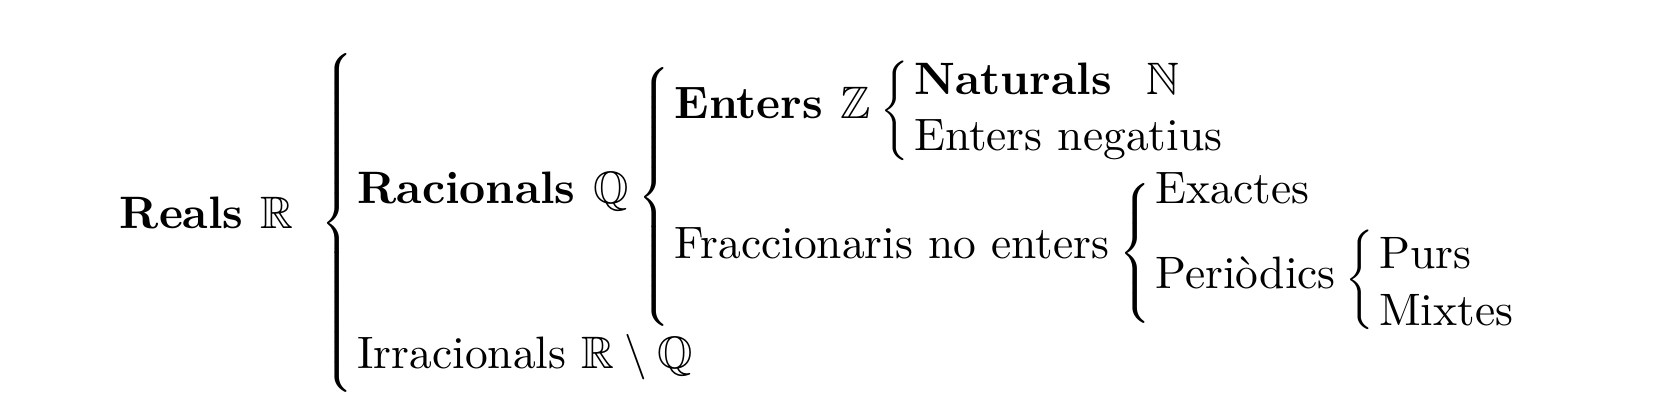
\includegraphics[max width=0.8\linewidth, max height=5cm]{../../../docs/nombres-reals/img/schema-conjunts-numerics.png}
\end{center}

Com veus, cada conjunt queda contingut dins del següent:

\[
\mathbb{N} \subset \mathbb{Z} \subset \mathbb{Q} \subset \mathbb{R}
\]

\begin{nota}{Inclusió}
Si $A \subset B$, tots els elements d'$A$ són també de $B$.

Exemple: $\mathbb{N} \subset \mathbb{Z}$.
\end{nota}

\section{La recta real: relació d'ordre}

\subsection{Relació d'ordre i desigualtats}

Donats dos nombres reals qualssevol, sempre en podem dir quin és més gran. Comencem per aquí:

\begin{definicio}{Definició: comparació de nombres reals}
Donats dos nombres reals $a$ i $b$, direm que $a$ és més gran que $b$, i ho escriurem $a>b$, si i només si

\[
a > b \;\;\Leftrightarrow\;\; a-b > 0.
\]
\end{definicio}

\begin{nota}{Més gran o igual vs. més gran}
Col·loquialment fem servir "més gran" tant per a $>$ com per a $\geq$, però matemàticament cal distingir-los:

\begin{enumerate}
\item \textbf{més gran} $\Rightarrow$ \emph{estrictament} més gran ($>$).
\item \textbf{més gran o igual} $\Rightarrow$ inclou el cas d'igualtat ($\geq$).
\end{enumerate}
\end{nota}

Amb aquesta idea, ja podem definir totes les relacions d'ordre possibles:

\begin{definicio}{Definició: relacions d'ordre en els reals}
Donats dos nombres reals $a$ i $b$:

\begin{center}
\begin{tabularx}{\linewidth}{lY}
\toprule
\textbf{Notació} & \textbf{Descripció i condició equivalent} \\
\midrule
$a=b$ & Igualtat: $a=b \Longleftrightarrow a-b=0$ \\
$a \geq b$ & "$a$ és més gran o igual que $b$": $a \geq b \Longleftrightarrow a-b \geq 0$ \\
$a \leq b$ & "$a$ és més petit o igual que $b$": $a \leq b \Longleftrightarrow a-b \leq 0$ \\
$a > b$ & "$a$ és més gran que $b$": $a > b \Longleftrightarrow a-b > 0$ \\
$a < b$ & "$a$ és més petit que $b$": $a < b \Longleftrightarrow a-b < 0$ \\
\bottomrule
\end{tabularx}
\end{center}
\end{definicio}

\begin{exemple}{\textbf{Exemple:} Relacions d'ordre}
Donats els nombres $-3$, $4$ i $6$:

\begin{center}
\begin{tabular}{lll}
\toprule
\textbf{Enunciat} & \textbf{Notació} & \textbf{Condició numèrica} \\
\midrule
$6$ és igual que $6$ & $6 = 6$ & $6-6=0$ és zero \\
$4$ és més petit o igual que $6$ & $4 \leq 6$ & $4-6=-2$ és negatiu \\
$4$ és més gran que $-3$ & $4 > -3$ & $4-(-3)=7$ és positiu \\
$-3$ és més petit que $4$ & $-3 < 4$ & $-3-4=-7$ és negatiu \\
\bottomrule
\end{tabular}
\end{center}
\end{exemple}

Fixa't que aquestes cinc relacions cobreixen totes les possibilitats: dos nombres reals sempre acaben lligats per una d'elles, i això és el que ens permetrà situar-los tots sobre una recta.

\subsection{Representació gràfica}

Per representar els nombres reals sobre una recta només ens calen dues referències: el $0$ i l'$1$, amb l'$1$ a la dreta del $0$. Aquesta distància marca la unitat i ens permet situar la resta d'enters, positius a la dreta i negatius a l'esquerra.

\begin{center}
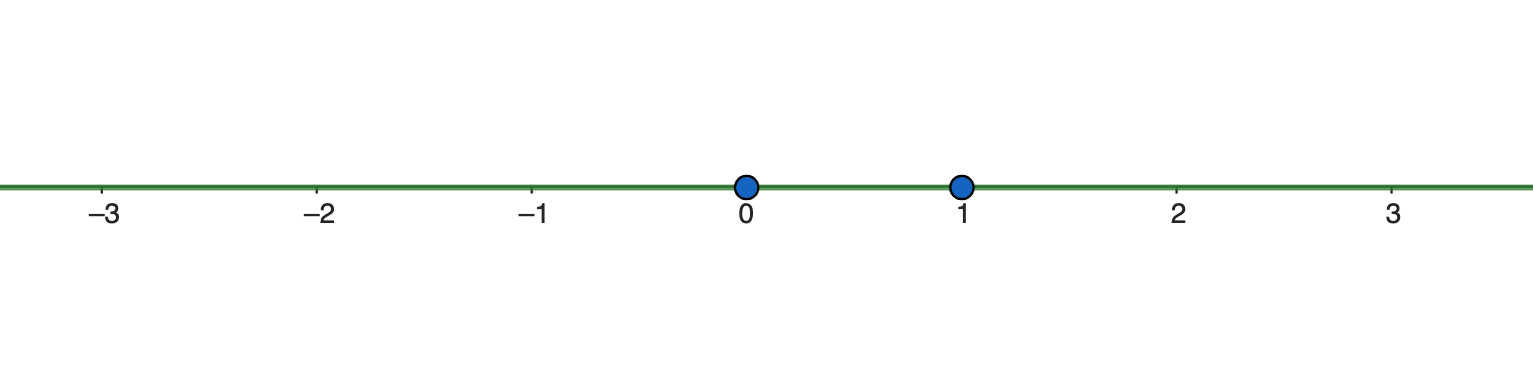
\includegraphics[max width=0.8\linewidth, max height=5cm]{../../../docs/nombres-reals/img/recta_real.png}
\end{center}

La regla és senzilla: com més gran és un nombre, més a la dreta el trobarem; com més petit, més a l'esquerra.

\begin{nota}{Escala de la recta real}
Recorda que en marcar el punt $1$ fixem l'escala de tota la recta: la distància de $0$ a $1$ determina la unitat i permet situar la resta de nombres.
\end{nota}

\begin{exemple}{\textbf{Exemple:} Representació de punts a la recta real}
Considerem els nombres reals $2$, $\pi$, $-\sqrt{2}$ i $\tfrac{21}{4}$. La seva representació decimal és:

\[
2 = 2{,}0, \qquad
\pi = 3{,}141592\dots, \qquad
-\sqrt{2} = -1{,}414213\dots, \qquad
\tfrac{21}{4} = 5{,}25.
\]

$\pi$ i $-\sqrt{2}$ són irracionals, així que no tenen una representació decimal exacta. Tot i això, els podem situar igualment a la recta real:

\begin{center}
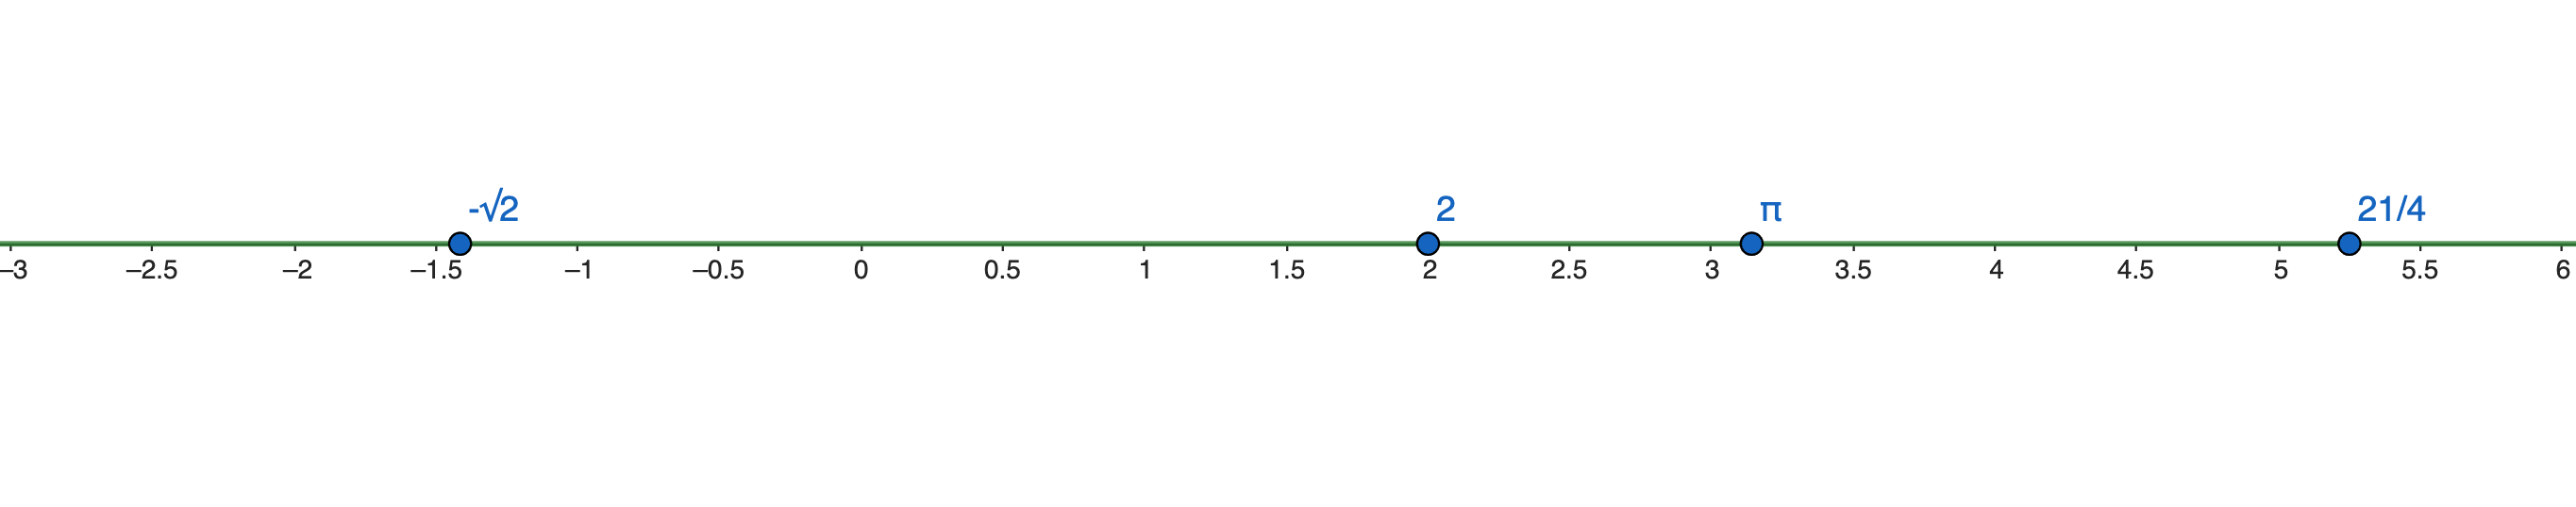
\includegraphics[max width=0.8\linewidth, max height=5cm]{../../../docs/nombres-reals/img/recta_real_exemple.png}
\end{center}
\end{exemple}

\begin{exemple}{\textbf{Exemple:} Comparació entre fracció i decimal}
Vegem que $\tfrac{2}{3} < 0{,}7$:

\[
\tfrac{2}{3} = 0{,}666\dots \quad < \quad 0{,}7.
\]
\end{exemple}

Amb la recta real i la relació d'ordre a punt, ja tenim el que ens cal per definir els \textbf{intervals} i el \textbf{valor absolut}, que veurem a continuació.

\section{Intervals i valor absolut}

A La recta real hem vist la relació d'ordre entre nombres reals. Ara la utilitzarem per definir dos conceptes que farem servir més endavant: els \textbf{intervals} i el \textbf{valor absolut}.

\subsection{Intervals}

Segur que ja coneixes els intervals de cursos anteriors: són conjunts de nombres que compleixen una condició d'ordre respecte a un o dos valors donats. Repassem-ho.

\begin{definicio}{Definició: interval obert i interval tancat}
Donats dos nombres reals $a$ i $b$ amb $a<b$, es defineix un \textbf{interval obert} com

\[
(a,b) = \{x\in \mathbb{R}, a<x<b\}
\]

i un \textbf{interval tancat} com

\[
[a,b] = \{x \in \mathbb{R}, a \leq x \leq b\}
\]

Sobre la recta real es representen així:

\begin{center}
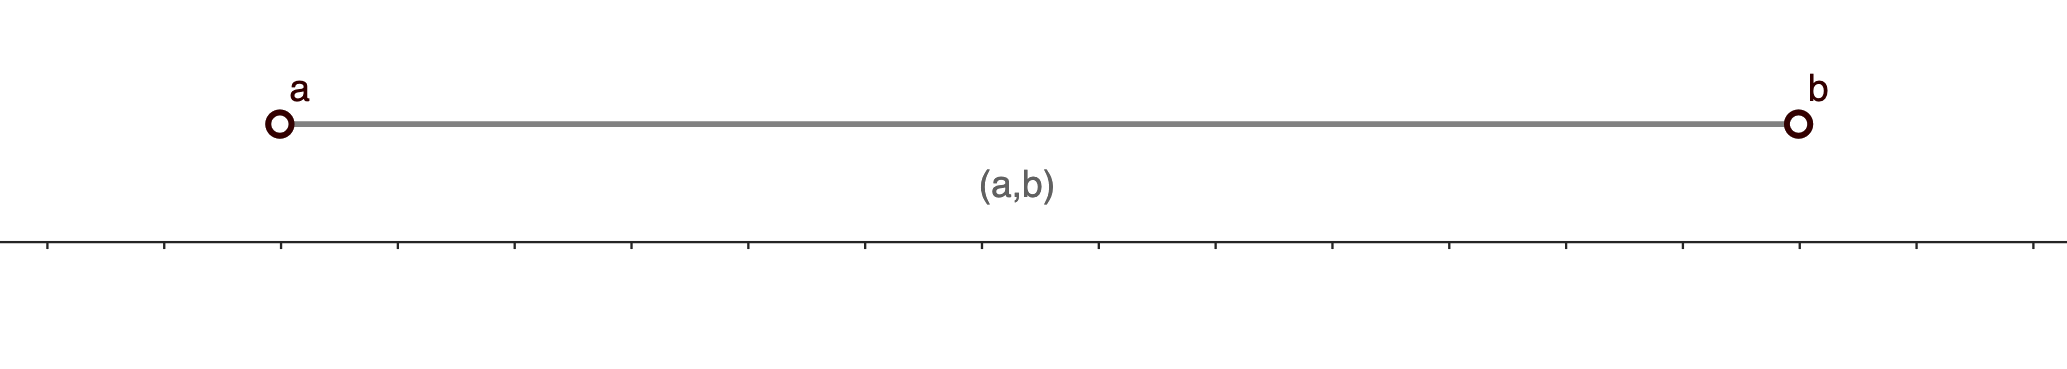
\includegraphics[max width=0.8\linewidth, max height=5cm]{../../../docs/nombres-reals/img/interval_obert.png}
\end{center}

\begin{center}
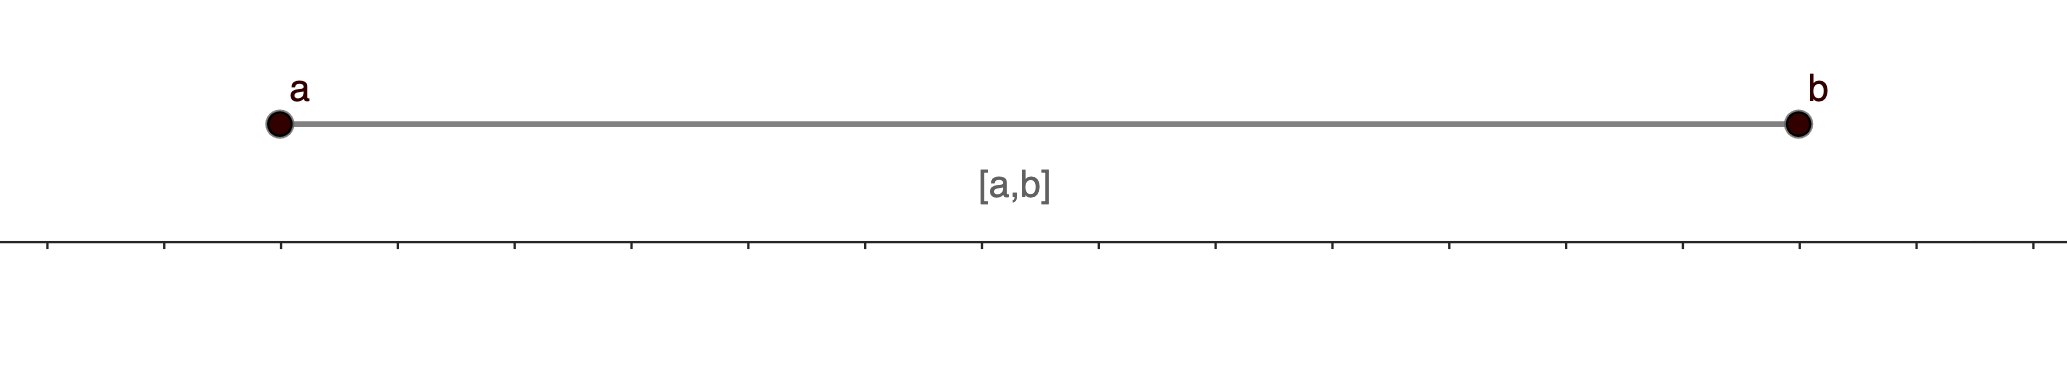
\includegraphics[max width=0.8\linewidth, max height=5cm]{../../../docs/nombres-reals/img/interval_tancat.png}
\end{center}
\end{definicio}

Però un interval no cal que sigui obert o tancat pels dos costats alhora. Si un extrem és obert i l'altre tancat, parlem d'un \textbf{interval semiobert} (o semitancat). Si un dels extrems és infinit, en diem \textbf{semirecta}:

\begin{center}
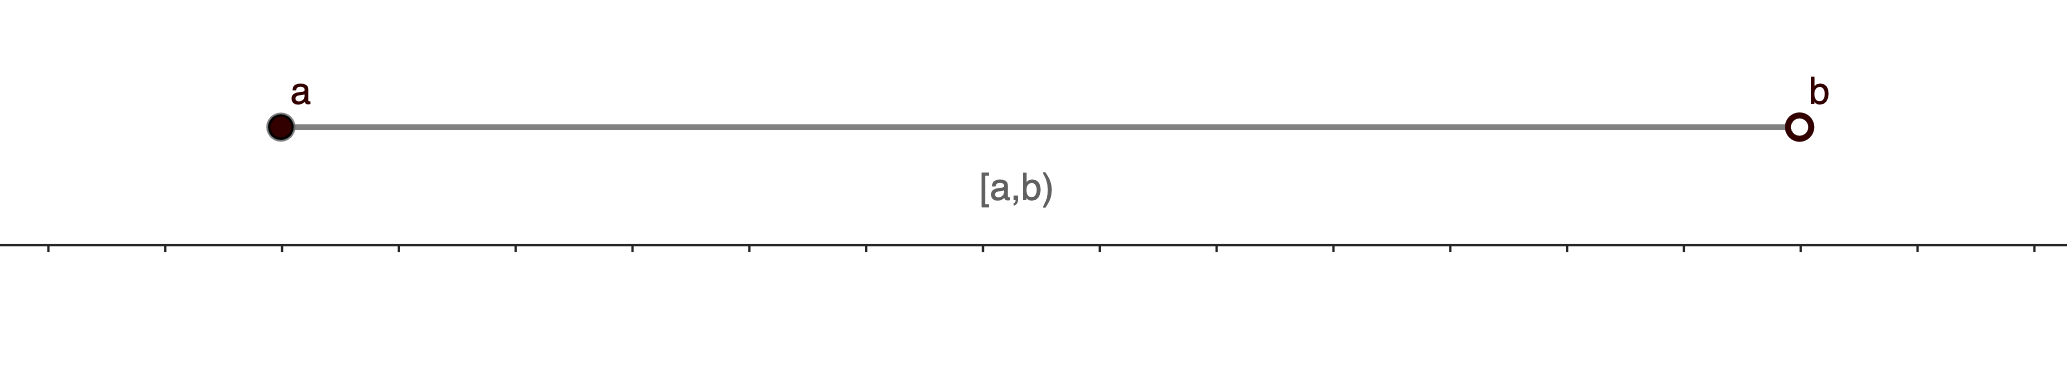
\includegraphics[max width=0.8\linewidth, max height=5cm]{../../../docs/nombres-reals/img/interval_semiobert.png}
\end{center}

\begin{center}
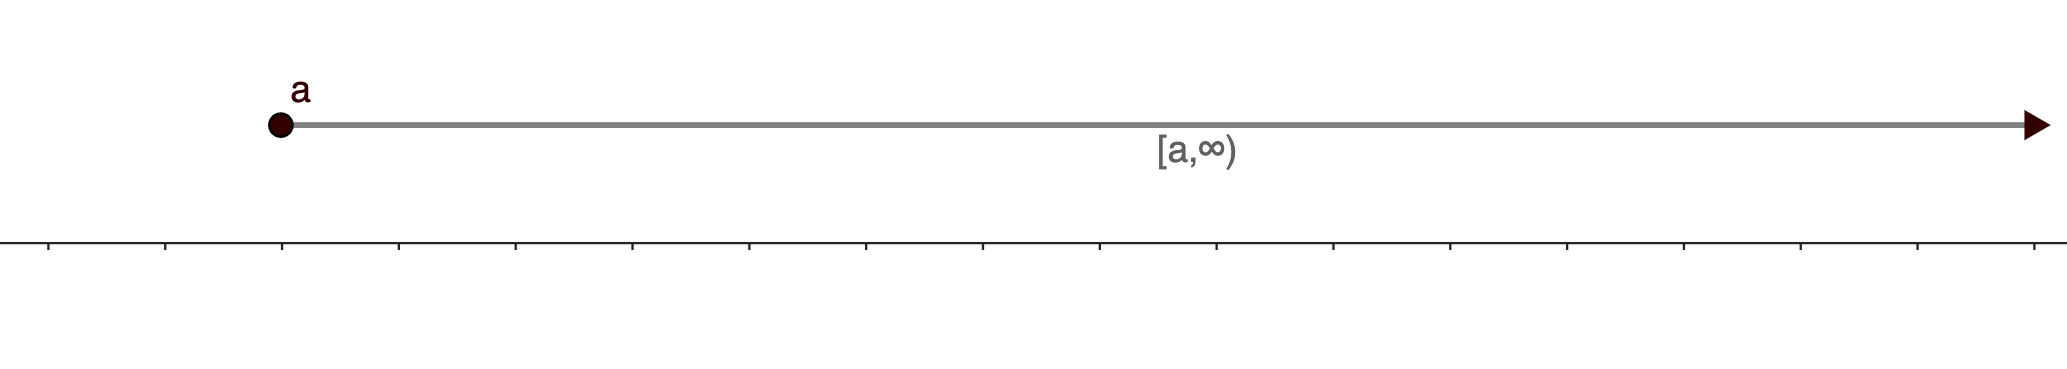
\includegraphics[max width=0.8\linewidth, max height=5cm]{../../../docs/nombres-reals/img/interval_semirecta.png}
\end{center}

Fixa't en aquesta taula: t'hi pots referir sempre que dubtis de com s'escriu cada tipus d'interval.

\begin{propietat}{Propietat: classificació dels intervals}
\begin{center}
\begin{tabular}{lll}
\toprule
\textbf{Notació} & \textbf{Nom} & \textbf{Condició} \\
\midrule
$(a,b)$ & Obert & $a < x < b$ \\
$[a,b]$ & Tancat & $a \leq x \leq b$ \\
$(a,b]$ & Semiobert a l'esquerra & $a < x \leq b$ \\
$[a,b)$ & Semiobert a la dreta & $a \leq x < b$ \\
$(a,+\infty)$ & Semirecta oberta & $x > a$ \\
$[a,+\infty)$ & Semirecta tancada & $x \geq a$ \\
$(-\infty,b)$ & Semirecta oberta & $x < b$ \\
$(-\infty,b]$ & Semirecta tancada & $x \leq b$ \\
\bottomrule
\end{tabular}
\end{center}
\end{propietat}

\subsection{Valor absolut}

Quan et cal treballar amb una quantitat sempre positiva, encara que el nombre de partida no ho sigui, entra en joc el \textbf{valor absolut}:

\begin{definicio}{Definició: valor absolut}
Donat un nombre real $a$, es defineix el seu valor absolut com

\[
|a| = \begin{cases} a & \text{ si } a \geq 0 \\ -a & \text{ si } a <0 \end{cases}
\]
\end{definicio}

\begin{exemple}{\textbf{Exemple:} Càlcul d'alguns valors absoluts}
\[
|3| = |+3| = 3 \qquad\qquad |-5| = -(-5) = 5
\]
\end{exemple}

Dit d'una altra manera: si el nombre ja és positiu, el deixem igual; si és negatiu, li canviem el signe.

Aquesta idea té una aplicació immediata: mesurar distàncies. Sobre la recta real, la distància entre dos punts $a$ i $b$ és $b-a$ si $a<b$, o $a-b$ si $a>b$. Fixa't que les dues expressions són oposades:

\begin{exemple}{\textbf{Exemple:} Càlcul d'algunes distàncies}
Siguin $a=3$ i $b=7$. Aleshores

\[
a-b = 3-7 = -4 \qquad\qquad b-a = 7-3 = 4
\]
\end{exemple}

Com que una distància mai és negativa, ens n'hi ha prou amb prendre el valor absolut d'una de les dues expressions, sense preocupar-nos de quin nombre és més gran:

\begin{definicio}{Definició: distància entre dos nombres reals}
Siguin $a$ i $b$ dos nombres reals qualssevol. Es defineix la distància entre $a$ i $b$ com

\[
d(a,b) = |b-a|
\]
\end{definicio}

Amb aquesta eina ens podem preguntar: quins nombres $x$ estan a una distància menor que un cert $r$ d'un nombre $a$? És a dir, quins $x$ compleixen

\[
d(a,x)<r
\]

Gràficament, es tracta de trobar els extrems d'un interval $(e_1,e_2)$:

\begin{center}
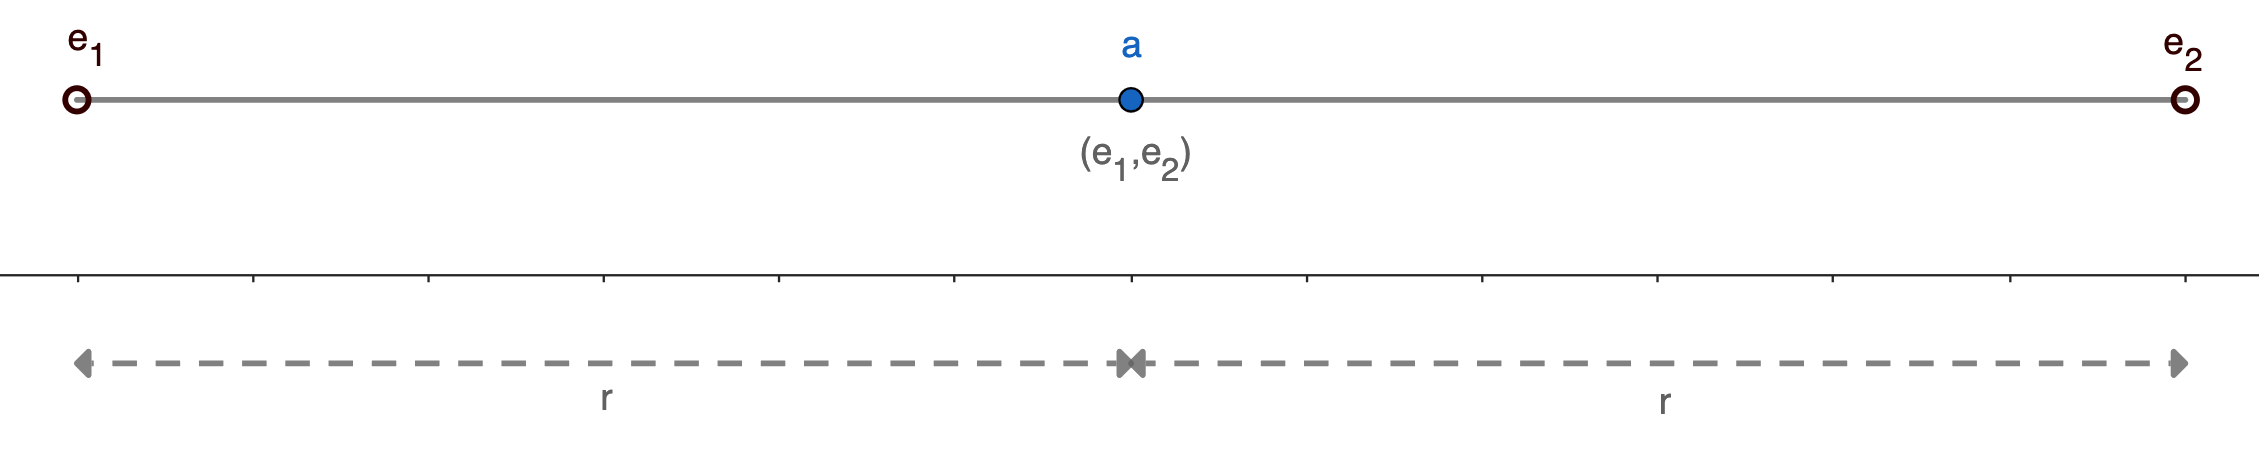
\includegraphics[max width=0.8\linewidth, max height=5cm]{../../../docs/nombres-reals/img/interval_entorn.png}
\end{center}

\begin{exemple}{\textbf{Exemple:} Reals a una distància menor que un valor conegut d'un altre real}
Sigui $a=4$ i $r=6$. Volem els punts la distància dels quals a $a$ sigui menor que $r$:

\[
d(x,4)<6 \qquad\Rightarrow\qquad |x-4|<6
\]

Gràficament, busquem els extrems del següent interval:

\begin{center}
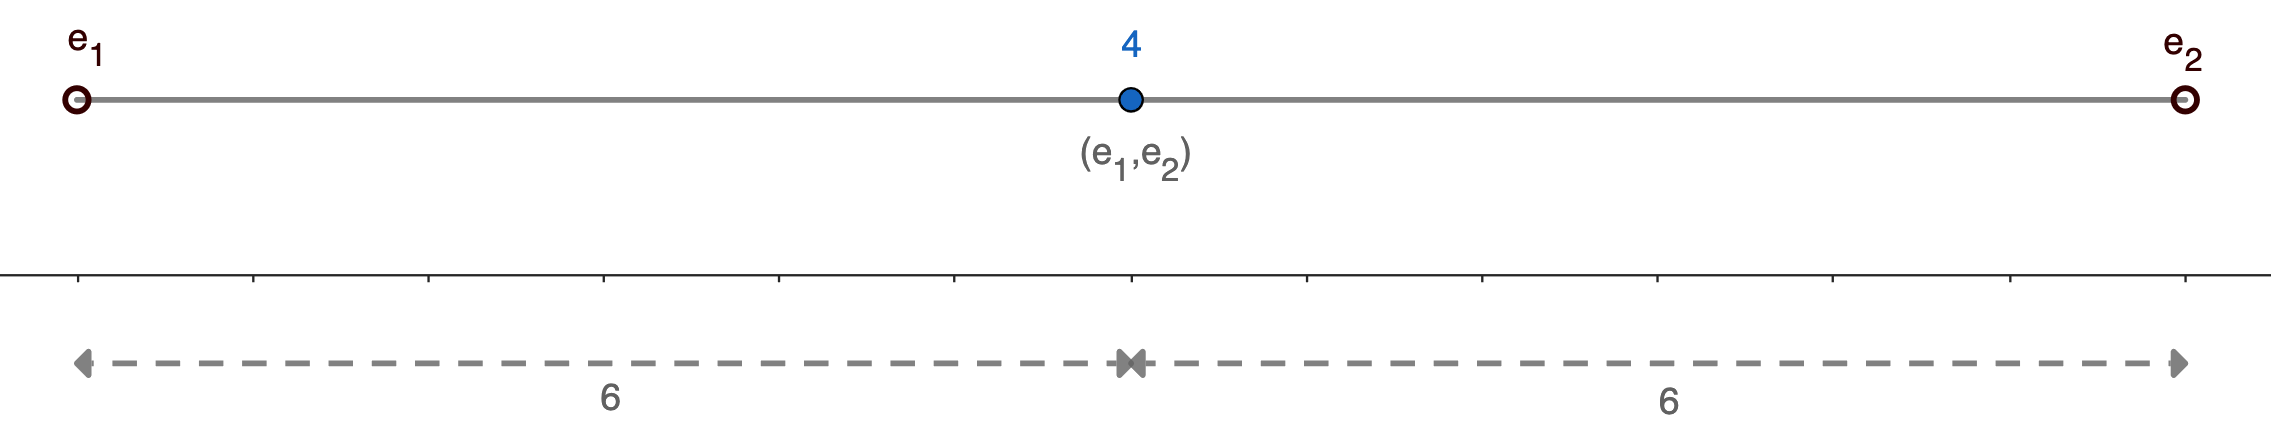
\includegraphics[max width=0.8\linewidth, max height=5cm]{../../../docs/nombres-reals/img/entorn_exemple.png}
\end{center}

Observem que $e_1=4-6=-2$ i $e_2=4+6=10$. Per tant, l'interval demanat és $(-2,10)$.
\end{exemple}

Aquest resultat es generalitza sempre igual, per a qualsevol punt i qualsevol distància:

\begin{propietat}{Propietat: entorn d'un punt}
Per a qualsevol $a \in \mathbb{R}$ i $r>0$ es té

\[
|x-a| < r \quad \Longleftrightarrow \quad a-r < x < a+r,
\]

és a dir, l'interval solució és sempre $(a-r,\,a+r)$.
\end{propietat}

Ens podem plantejar ara la pregunta contrària: quins punts són \textbf{lluny} d'$a$, és a dir, a una distància \textbf{més gran} que $r$? No cal cap tècnica nova: n'hi ha prou de resoldre la condició de sempre i quedar-nos amb tot el que en queda fora.

\begin{propietat}{Propietat: punts a distància més gran que un valor}
Per a qualsevol $a \in \mathbb{R}$ i $r>0$ es té

\[
|x-a| > r \quad \Longleftrightarrow \quad x < a-r \ \text{ o } \ x > a+r,
\]

és a dir, la solució no és un interval, sinó la unió de dues semirectes: $(-\infty,\,a-r)\cup(a+r,\,+\infty)$.
\end{propietat}

\begin{nota}{D'on surt: el complementari}
Qualsevol punt de la recta compleix exactament una d'aquestes tres coses: o és a distància menor que $r$ d'$a$, o hi és exactament a distància $r$, o hi és a distància més gran. Els dos primers casos formen l'interval tancat $[a-r,\,a+r]$, que és la solució de $|x-a|\leq r$.

Els punts que busquem, doncs, són \textbf{tots els altres}: el complementari d'aquest interval. I fixa't en un detall important: en passar al complementari, els extrems canvien de tipus. Els punts $a-r$ i $a+r$ són exactament a distància $r$, així que no compleixen la desigualtat estricta i queden fora de la solució; per això l'interval tancat es converteix en dues semirectes \textbf{obertes}.
\end{nota}

\begin{exemple}{\textbf{Exemple:} Punts a distància més gran que $2$ del punt $3$}
Volem resoldre $|x-3|>2$.

Primer resolem la condició contrària, tal com hem fet fins ara:

\[
|x-3|\leq 2 \qquad\Rightarrow\qquad 1 \leq x \leq 5
\]

La solució d'aquesta és l'interval $[1,5]$. Els punts que busquem són els que en queden fora:

\[
(-\infty,1)\cup(5,+\infty)
\]

Comprovem-ho amb dos valors concrets: $x=6$ dona $|6-3|=3$, que sí que és més gran que $2$; en canvi $x=1$ dona $|1-3|=2$, que \textbf{no} és més gran que $2$, i per això l'extrem queda exclòs.
\end{exemple}

\subsection{Inequacions lineals}

Una inequació lineal és una desigualtat amb una incògnita on les expressions implicades són polinomis de grau $1$. Ja les vas resoldre en cursos anteriors i el mètode és pràcticament el mateix que amb les equacions de primer grau... amb una diferència important que cal vigilar.

\begin{exemple}{\textbf{Exemple:} Resolució d'una inequació lineal}
\[
2x-5>7
\]

Aïllem la $x$ igual que amb les equacions de primer grau:

\[
2x > 7 + 5 \qquad\Rightarrow\qquad 2x > 12 \qquad\Rightarrow\qquad x > \frac{12}{2} = 6
\]

Per tant, la solució és la semirecta $(6,+\infty)$.
\end{exemple}

\begin{nota}{Atenció amb el signe!}
Quan multipliques o divideixes una desigualtat per un nombre negatiu, cal \textbf{canviar el sentit de la desigualtat}.

Per exemple: $2 < 5 \quad \Longrightarrow \quad -2 > -5$
\end{nota}

\begin{exemple}{\textbf{Exemple:} Resolució d'una altra inequació lineal}
\[
-3x + 5 \leq 23
\]

\[
-3x \leq 23 - 5 \qquad\Rightarrow\qquad -3x \leq 18
\]

El valor que passem dividint és negatiu: girem el sentit de la desigualtat (només cal fer-ho amb el producte i la divisió):

\[
x \geq \frac{18}{-3} = -6
\]

Per tant, la solució és la semirecta $[-6,+\infty)$.
\end{exemple}

\section{Aproximacions i errors}

Molts nombres reals —els irracionals— tenen infinites xifres decimals que no es repeteixen mai. Per tant, mai els podem escriure ni operar-hi de manera exacta. Altres cops, independentment de com siguin els nombres reals, treballem amb una precisió limitada i això ens porta a l'\textbf{aproximació} de valors.

\subsection{Aproximació d'un nombre}

Per aproximar un nombre a un cert nombre de xifres decimals tenim dues estratègies bàsiques: el \textbf{truncament} i l'\textbf{arrodoniment}. Vegem en què consisteix cadascuna.

\begin{definicio}{Definició: truncament}
Truncar un nombre a $n$ xifres decimals vol dir eliminar totes les xifres a partir de la posició $n+1$, sense tocar les que queden.
\end{definicio}

\begin{definicio}{Definició: arrodoniment}
Arrodonir un nombre a $n$ xifres decimals vol dir fixar-se en la xifra que ocupa la posició $n+1$:

\begin{itemize}
\item Si és $5$ o més, sumem una unitat a l'última xifra que conservem.
\item Si és menor que $5$, l'última xifra que conservem no canvia.
\end{itemize}
\end{definicio}

\begin{exemple}{\textbf{Exemple:} Truncament i arrodoniment de $\pi$}
Considerem $\pi = 3{,}14159265\ldots$

\begin{center}
\begin{tabular}{lll}
\toprule
\textbf{Xifres decimals} & \textbf{Truncament} & \textbf{Arrodoniment} \\
\midrule
2 & $3{,}14$ & $3{,}14$ \\
4 & $3{,}1415$ & $3{,}1416$ \\
\bottomrule
\end{tabular}
\end{center}

Fixa't que a 4 decimals la cinquena xifra de $\pi$ és un $9$: per això l'arrodoniment puja l'última xifra ($5 \to 6$), mentre que el truncament simplement la descarta.
\end{exemple}

\begin{nota}{Xifres significatives}
Les \emph{xifres significatives} d'un nombre són totes les que aporten informació sobre la seva precisió, comptant des de la primera xifra diferent de zero. Per exemple, $0{,}00530$ en té tres ($5$, $3$ i $0$): els zeros inicials només col·loquen la coma.
\end{nota}

\subsection{Error absolut i error relatiu}

Quan canviem un valor exacte $x$ per una aproximació $x'$, cometem un \textbf{error}. I ens interessa poder mesurar-lo.

\begin{definicio}{Definició: error absolut}
Si $x$ és el valor exacte d'una magnitud i $x'$ n'és una aproximació, l'\textbf{error absolut} és

\[
E_a = |x - x'|
\]
\end{definicio}

\begin{exemple}{\textbf{Exemple:} Error absolut de l'aproximació de $\pi$}
Si aproximem $\pi \approx 3{,}14$:

\[
E_a = |\pi - 3{,}14| = |3{,}14159\ldots - 3{,}14| = 0{,}00159\ldots
\]
\end{exemple}

L'error absolut es mesura en les mateixes unitats que la magnitud, però per si sol no ens diu si l'aproximació és bona o dolenta: un error d'1 metre és insignificant mesurant la distància entre ciutats, però enorme mesurant el gruix d'un llibre. Per això ens cal l'\textbf{error relatiu}.

\begin{definicio}{Definició: error relatiu}
L'\textbf{error relatiu} és el quocient entre l'error absolut i el valor absolut del valor exacte:

\[
E_r = \frac{E_a}{|x|} = \frac{|x-x'|}{|x|}
\]

Sovint s'expressa en tant per cent, multiplicant per $100$.
\end{definicio}

\begin{exemple}{\textbf{Exemple:} Comparació de dues aproximacions amb el mateix error absolut}
Imaginem dues mesures, totes dues amb un error absolut d'$1\,\text{m}$:

\begin{itemize}
\item Distància entre ciutats: $x = 100\,\text{km} = 100\,000\,\text{m}$, amb $E_r = \dfrac{1}{100\,000} = 0{,}001\%$.
\item Llargada d'una taula: $x = 2\,\text{m}$, amb $E_r = \dfrac{1}{2} = 50\%$.
\end{itemize}

Mateix error absolut, però resultats ben diferents: l'error relatiu deixa clar que un metre és insignificant en 100 km, però inacceptable en la llargada d'una taula.
\end{exemple}

\begin{nota}{Cota de l'error en un arrodoniment}
En arrodonir a $n$ xifres decimals, l'error absolut mai supera mitja unitat de l'última xifra conservada. Per exemple, arrodonint a les centèsimes ($n=2$), l'error no supera $0{,}005$.
\end{nota}

\begin{exemple}{\textbf{Exemple:} Comprovació de la cota en arrodonir}
Arrodonim $x = 8{,}2793$ a les centèsimes: $x' = 8{,}28$.

\[
E_a = |8{,}2793 - 8{,}28| = 0{,}0007 \leq 0{,}005
\]

Ara mirem el cas més desfavorable: $x = 8{,}275$. Com que la tercera xifra decimal és un $5$, arrodonim a $x' = 8{,}28$, i llavors

\[
E_a = |8{,}275 - 8{,}28| = 0{,}005
\]

Aquí l'error \textbf{iguala} la cota: per això en diem cota, un màxim que mai se supera però que sí que es pot arribar a assolir.
\end{exemple}

\begin{exemple}{\textbf{Exemple:} Acotar el valor real a partir d'un arrodoniment}
Un cronòmetre marca $12{,}4\,\text{s}$, arrodonits a la dècima. Quin marge de valors pot tenir el temps real $t$?

Com que l'arrodoniment és a $n=1$ xifra decimal, la cota de l'error és $0{,}5 \cdot 10^{-1} = 0{,}05$:

\[
|t - 12{,}4| \leq 0{,}05
\]

Això dona, en principi, $12{,}35 \leq t \leq 12{,}45$. Però cal vigilar l'extrem superior: si $t=12{,}45$, la xifra de les centèsimes és un $5$ i arrodoneix cap amunt, $12{,}45 \to 12{,}5$, no a $12{,}4$. Aquest valor, doncs, no arrodoneix a $12{,}4$ i queda fora:

\[
12{,}35 \leq t < 12{,}45
\]

Dit amb notació d'interval:

\[
t \in [12{,}35,\ 12{,}45)
\]

Fixa't en el paral·lelisme amb l'entorn d'un punt de Intervals i valor absolut: allà buscàvem els $x$ a una distància menor que $r$ d'un punt $a$, és a dir $|x-a|<r \Leftrightarrow x \in (a-r,\,a+r)$, un interval sempre obert pels dos costats. Aquí el plantejament és el mateix —una distància màxima respecte d'un valor central—, però com que la igualtat sí que es pot arribar a donar en un dels costats (i no en l'altre, per la regla d'arrodoniment), l'interval resultant és semiobert enlloc de totalment obert.
\end{exemple}

\section{Potències}

\subsection{Definició}

Ja coneixes les potències de cursos anteriors: és un concepte que hem anat ampliant curs rere curs a conjunts numèrics cada cop més grans.

\begin{nota}{Notació: potència}
La notació utilitzada per a les potències és

\[
a^n
\]

on $a$ s'anomena \textbf{base} i $n$ \textbf{exponent}.
\end{nota}

Quan l'exponent és natural, la idea és senzilla: multipliquem $a$ tants cops com indiqui l'exponent.

\begin{definicio}{Definició: potència d'exponent natural}
Si $a$ és un nombre real i $n$ un nombre natural, aleshores

\[
a^n = \underbrace{a \cdot a \cdot \dots \cdot a}_n
\]
\end{definicio}

\begin{exemple}{\textbf{Exemple:} Bases positives i negatives}
\[
3^5 = \underbrace{3\cdot 3\cdot 3\cdot 3\cdot 3}_5 = 243,
\qquad
(-2)^4 = \underbrace{(-2)\cdot(-2)\cdot(-2)\cdot(-2)}_4 = 16.
\]
\end{exemple}

\begin{nota}{Atenció amb els parèntesis}
No és el mateix $-2^4$ que $(-2)^4$:

\begin{enumerate}
\item $-2^4=-(2^4)=-16$
\item $(-2)^4=16$
\end{enumerate}
\end{nota}

\subsection{Propietats i exemples: exponents naturals}

Amb exponents naturals, les potències compleixen algunes propietats bàsiques. Ens serviran de punt de partida quan, més endavant, estenguem la definició a l'exponent zero i als exponents negatius.

\begin{propietat}{Propietat: producte de potències de la mateixa base}
Si $m,n\in\mathbb{N}$, aleshores

\[
a^m \cdot a^n = a^{m+n}, \qquad a \in \mathbb{R}.
\]
\end{propietat}

\begin{exemple}{\textbf{Exemple}}
\[
2^3 \cdot 2^4 = (2\cdot 2\cdot 2)\cdot(2\cdot 2\cdot 2\cdot 2).
\]

Comptant tots els factors en tenim 7, tots iguals a 2:

\[
2^3 \cdot 2^4 = 2^7 = 128.
\]

Comprova-ho: $2^3=8$, $2^4=16$, i $8\cdot 16 = 128$.
\end{exemple}

\begin{propietat}{Propietat: quocient de potències de la mateixa base}
Si $m,n\in\mathbb{N}$ amb $m> n$, aleshores

\[
\frac{a^m}{a^n} = a^{m-n}, \qquad a \in \mathbb{R},\; a \neq 0.
\]
\end{propietat}

\begin{exemple}{\textbf{Exemple}}
\[
\frac{5^6}{5^2}=\frac{5\cdot 5\cdot 5\cdot 5\cdot 5\cdot 5}{5\cdot 5}
=5\cdot 5\cdot 5\cdot 5 = 5^4 = 625.
\]

Comprova-ho: $5^6=15\,625$, $5^2=25$ i $\tfrac{15\,625}{25}=625$.
\end{exemple}

\begin{nota}{Atenció}
Amb exponents naturals, aquesta regla només val si $m> n$. Què passa si $m\leq n$? Ho resoldrem més endavant amb l'exponent negatiu i l'exponent $0$.
\end{nota}

\begin{propietat}{Propietat: potència d'una potència}
Si $m,n\in\mathbb{N}$, aleshores

\[
\left(a^m\right)^n = a^{m \cdot n}, \qquad a \in \mathbb{R}.
\]
\end{propietat}

\begin{exemple}{\textbf{Exemple}}
\[
\left(3^2\right)^4 = \left(9\right)^4 = 6561, \qquad\text{i també}\qquad 3^{2\cdot 4}=3^8=6561.
\]
\end{exemple}

\subsection{Extensió de la definició}

Aquestes propietats funcionen bé mentre l'exponent és natural. Però volem que continuïn essent vàlides quan els exponents s'igualen ($m=n$) o quan el numerador és més petit que el denominador ($m<n$). Per això ens cal ampliar la definició de potència als casos d'exponent zero i d'exponent negatiu.

\begin{definicio}{Definició: potència d'exponent zero}
Si $a$ és un nombre real diferent de zero, definim

\[
a^0 = 1.
\]
\end{definicio}

\begin{nota}{Justificació del cas $a^0$}
Perquè la regla del quocient es mantingui:

\[
a^0 = a^{n-n} = \frac{a^n}{a^n} = 1, \qquad a\neq 0.
\]

(El valor $0^0$ queda fora d'aquesta definició: no està definit, és una indeterminació.)
\end{nota}

\begin{definicio}{Definició: potència d'exponent negatiu}
Si $a$ és un nombre real diferent de zero i $n\in\mathbb{N}$, definim

\[
a^{-n} = \frac{1}{a^n}.
\]
\end{definicio}

\begin{nota}{Justificació del cas amb exponent negatiu}
Perquè la regla del producte es mantingui:

\[
1 = a^0 = a^{n-n} = a^{n} \cdot a^{-n}.
\]

D'aquí surt que $a^{-n}$ ha de valer $\tfrac{1}{a^n}$.
\end{nota}

\begin{exemple}{\textbf{Exemple:} Ús d'exponents zero i negatius}
\[
5^0 = 1, \qquad 7^{-2} = \frac{1}{7^2} = \frac{1}{49}.
\]

Un càlcul combinat:

\[
\frac{4^3 \cdot 4^{-5}}{4^0} = 4^{3+(-5)-0} = 4^{-2} = \frac{1}{16}.
\]
\end{exemple}

Amb aquestes dues definicions, totes les propietats anteriors segueixen valent, ara per a exponents enters.

\begin{definicio}{Definició: potència amb exponent enter (definició global)}
Per a tot $a\in\mathbb{R}$ i $n\in\mathbb{Z}$, definim

\[
a^n=
\begin{cases}
\underbrace{a\cdot a \cdot \ldots \cdot a}_{n\text{ factors}}, & n\in\mathbb{N},\\[6pt]
1, & n=0,\ a\neq 0,\\[6pt]
\dfrac{1}{a^{-n}}, & n<0,\ a\neq 0.
\end{cases}
\]
\end{definicio}

A partir d'ara, les propietats que hem vist segueixen essent vàlides per a qualsevol exponent enter, sempre que no comportin dividir per zero.

\subsection{Propietats i exemples: exponents enters}

Recordem les propietats anteriors, ara vàlides per a exponents enters, amb un exemple per cadascuna.

\begin{propietat}{Propietat: producte de potències de la mateixa base}
\[
a^m \cdot a^n = a^{m+n}, \qquad a \in \mathbb{R},\; a \neq 0.
\]
\end{propietat}

\begin{exemple}{\textbf{Exemple}}
\[
2^{-3}\cdot 2^{5}=2^{-3+5}=2^2=4.
\]

Comprova-ho: $\tfrac{1}{2^3}\cdot 2^5=\tfrac{1}{8}\cdot 32=4$.
\end{exemple}

\begin{nota}{Importància del fet que $a\neq 0$}
Si $a=0$ i algun exponent és negatiu, la potència no està definida. Per exemple:

\[
0^{5}\cdot 0^{-7} =0^{-2}=\frac{1}{0^2}= \frac{1}{0},
\]

que no té sentit. Excloent $a=0$ ens assegurem que la propietat sigui sempre vàlida.
\end{nota}

\begin{propietat}{Propietat: quocient de potències de la mateixa base}
\[
\frac{a^m}{a^n} = a^{m-n}, \qquad a \in \mathbb{R},\; a \neq 0.
\]
\end{propietat}

\begin{exemple}{\textbf{Exemple}}
\[
\frac{5^2}{5^{-3}} = 5^{2-(-3)}=5^5=3125.
\]

També: $\tfrac{25}{1/125}=3125$.
\end{exemple}

\begin{propietat}{Propietat: potència d'una potència}
\[
\left(a^m\right)^n = a^{m \cdot n}, \qquad a \in \mathbb{R},\; a \neq 0.
\]
\end{propietat}

\begin{exemple}{\textbf{Exemple}}
\[
\left(3^{-2}\right)^3 = 3^{-6} = \frac{1}{729}.
\]

També: $\left(\tfrac{1}{9}\right)^3=\tfrac{1}{729}$.
\end{exemple}

\begin{nota}{Atenció als parèntesis}
No és el mateix $\left(a^m\right)^n$ que $a^{m^n}$:

\begin{enumerate}
\item $\left(2^2\right)^3 = 2^6 = 64$
\item $2^{2^3}=2^{8}=256$
\end{enumerate}
\end{nota}

\begin{propietat}{Propietat: potència d'exponent 1}
\[
a^1 = a, \qquad a \in \mathbb{R}.
\]
\end{propietat}

\begin{exemple}{\textbf{Exemple}}
\[
(-7)^1 = -7.
\]
\end{exemple}

\begin{propietat}{Propietat: potència d'un producte}
\[
(a \cdot b)^n = a^n \cdot b^n, \qquad a,b \in \mathbb{R},\; ab\neq 0.
\]
\end{propietat}

\begin{exemple}{\textbf{Exemple}}
\[
(2\cdot 3)^{-2} = 6^{-2} = \frac{1}{36}
\quad\text{i}\quad
2^{-2}\cdot 3^{-2} = \tfrac{1}{4}\cdot \tfrac{1}{9}=\tfrac{1}{36}.
\]
\end{exemple}

\begin{nota}{Compte}
Aquesta propietat no val per a sumes: $(a+b)^n \neq a^n+b^n$.
\end{nota}

\begin{propietat}{Propietat: potència d'un quocient}
\[
\left(\frac{a}{b}\right)^n = \frac{a^n}{b^n}, \qquad a,b \in \mathbb{R},\; b\neq 0.
\]
\end{propietat}

\begin{exemple}{\textbf{Exemple}}
\[
\left(\frac{2}{5}\right)^{-3} = \left(\frac{5}{2}\right)^3=\frac{125}{8},
\quad\text{i també}\quad \frac{2^{-3}}{5^{-3}}=\frac{1/8}{1/125}=\frac{125}{8}.
\]
\end{exemple}

\begin{nota}{Consell}
Recorda posar parèntesis a tota la fracció. No és el mateix

\[
\left(\tfrac{2}{5}\right)^3 = \tfrac{2^3}{5^3} = \tfrac{8}{125}
\]

que

\[
{\tfrac{2}{5}}^3 = \tfrac{2^3}{5}= \frac{8}{5}.
\]
\end{nota}

\subsection{Exemples finals}

Vegem-ho tot plegat amb un parell d'exemples que combinen diverses propietats.

\begin{exemple}{\textbf{Exemple:} Operació amb fraccions i variables}
\[
\begin{aligned}
\left(\frac{9x}{2}\right)^3 &= \frac{(9 \cdot x)^3}{2^3} \\
&= \frac{9^3 \cdot x^3}{2^3} \\
&= \frac{\left(3^2\right)^3 \cdot x^3}{2^3} \\
&= \frac{3^6 \cdot x^3}{2^3} \\
&= \frac{3^6}{2^3}x^3 \\
&= \frac{729}{8} x^3
\end{aligned}
\]

(Hem aplicat, en ordre, la potència d'un quocient, la potència d'un producte i la potència d'una potència.)
\end{exemple}

\begin{exemple}{\textbf{Exemple:} Descomposició en factors primers}
\[
\begin{aligned}
\frac{(12)^2 \cdot (9)^3}{(8)^{-4}} &= \frac{\left(2^2 \cdot 3\right)^2 \cdot \left(3^2\right)^3}{\left(2^3\right)^{-4}} \\
&= \frac{\left(2^2\right)^2\cdot 3^2 \cdot \left(3^2\right)^3}{\left(2^3\right)^{-4}} \\
&= \frac{2^4 \cdot 3^2 \cdot 3^6}{2^{-12}} \\
&= 2^4 \cdot 3^2 \cdot 3^6 \cdot 2^{12} \\
&= 2^{4+12} \cdot 3^{2+6} = 2^{16} \cdot 3^{8}
\end{aligned}
\]
\end{exemple}

\begin{exemple}{\textbf{Exemple:} Massa atòmica de l'hidrogen}
L'àtom d'hidrogen (H) té una massa de $1{,}66\cdot10^{-24}\,\text{g}$ (la \emph{massa atòmica}, és a dir, la massa d'un sol àtom). Quants àtoms calen per obtenir $10\,\text{kg}$ d'aquest gas? Usem la massa atòmica com a \textbf{factor de conversió} entre grams i nombre d'àtoms:

\[
\begin{aligned}
10\,\text{kg}\cdot\frac{1000\,\text{g}}{1\,\text{kg}}\cdot\frac{1\ \text{àtom}}{1{,}66\cdot10^{-24}\,\text{g}}
&= \frac{10^{4}}{1{,}66\cdot10^{-24}}\ \text{àtoms} \\
&=\ \frac{10^{4}\cdot10^{24}}{1{,}66}\ \text{àtoms} \\
&=\ \frac{1}{1{,}66}\cdot10^{28}\ \text{àtoms} \\
&\approx 0{,}6024\cdot10^{28}\ \text{àtoms} \\
&= \boxed{6{,}024\cdot10^{27}\ \text{àtoms}}
\end{aligned}
\]
\end{exemple}

\subsection{Annex: notació científica}

Una de les aplicacions més útils de les potències és escriure nombres molt grans o molt petits de manera compacta amb la \textbf{notació científica}, on l'exponent de $10$ indica l'\textbf{ordre de magnitud} i ens permet comparar mides ràpidament: com més gran l'exponent, més gran el nombre. Un nombre està en notació científica quan té la forma

\[
a \cdot 10^n, \qquad 1 \leq a < 10, \quad n \in \mathbb{Z}.
\]

\begin{exemple}{\textbf{Exemple:} Notació científica}
\[
0{,}000\,45 = 4{,}5 \cdot 10^{-4}, \qquad 72\,300 = 7{,}23 \cdot 10^{4}.
\]
\end{exemple}

\begin{nota}{Consell pràctic}
En càlculs amb notació científica, separa els factors numèrics dels factors de potències de 10:

\[
(a\cdot 10^m)(b\cdot 10^n) = (a\cdot b)\cdot 10^{m+n}.
\]

Recorda que el factor numèric ha de quedar entre $1$ i $10$; si $a\cdot b$ no ho compleix, reescriu el resultat.
\end{nota}

\begin{exemple}{\textbf{Exemple:} Càlcul amb notació científica}
\[
\begin{aligned}
\frac{(6{,}0\cdot 10^{-3})(8{,}0\cdot 10^{7})}{2{,}0\cdot 10^{2}}
&=\frac{6{,}0\cdot 8{,}0}{2{,}0}\cdot 10^{-3+7-2} \\
&=24\cdot 10^{2} \\
&=2{,}4\cdot 10^{3}.
\end{aligned}
\]
\end{exemple}

\begin{exemple}{\textbf{Exemple:} Comparació d'ordres de magnitud}
La massa de la Terra és aproximadament $5{,}97 \cdot 10^{24}\ \text{kg}$ i la de la Lluna, $7{,}35 \cdot 10^{22}\ \text{kg}$: només comparant els exponents ja ho veiem, $10^{24}$ és cent vegades més gran que $10^{22}$, així que la Terra pesa unes 100 vegades més que la Lluna.
\end{exemple}

\begin{exemple}{\textbf{Exemple:} Distàncies astronòmiques en notació científica}
La distància mitjana de la Terra al Sol és aproximadament

\[
149\,600\,000\ \text{km} = 1{,}496 \cdot 10^{8}\ \text{km}.
\]

La distància a l'estrella més propera (Pròxima Centauri) és d'uns

\[
40\,000\,000\,000\,000\ \text{km} \approx 4{,}0 \cdot 10^{13}\ \text{km}.
\]

Fixa't com els exponents $10^8$ i $10^{13}$ ja ens diuen que la distància a Pròxima Centauri és unes $10^5$ vegades més gran que la de la Terra al Sol.
\end{exemple}

\subsection{Taula resum}

\begin{center}
\begin{tabular}{ll}
\toprule
\textbf{Propietat} & \textbf{Fórmula} \\
\midrule
Producte de potències & $a^m \cdot a^n = a^{m+n}$ \\
Quocient de potències & $\dfrac{a^m}{a^n} = a^{m-n}$ \\
Potència d'una potència & $(a^m)^n = a^{m\cdot n}$ \\
Exponent zero & $a^0 = 1,\ a\neq 0$ \\
Exponent negatiu & $a^{-n} = \dfrac{1}{a^n}$ \\
Exponent 1 & $a^1 = a$ \\
Potència d'un producte & $(a\cdot b)^n = a^n\cdot b^n$ \\
Potència d'un quocient & $\left(\dfrac{a}{b}\right)^n = \dfrac{a^n}{b^n}$ \\
Notació científica & $a\cdot 10^n,\ 1\le a<10,\ n\in\mathbb{Z}$ \\
\bottomrule
\end{tabular}
\end{center}

\section{Arrels i radicals}

\subsection{Definició}

Ja saps elevar un nombre a una potència. Ara ens plantegem la pregunta inversa: quin nombre, elevat a $n$, dona un resultat $a$ conegut? En forma d'equació: $x^n=a$, les solucions són exactament el concepte d'arrel.

\begin{definicio}{Definició: arrel enèsima}
Siguin $a \in \mathbb{R}$ i $n \in \mathbb{N}$, amb $n>0$. Diem que $b$ és una \textbf{arrel enèsima} de $a$ si es compleix

\[
b^n = a.
\]

És a dir: un nombre real que, elevat a $n$, ens torna $a$.
\end{definicio}

\begin{exemple}{\textbf{Exemple:} quantes solucions té l'equació $x^n=a$?}
\begin{itemize}
\item $x^2=9$ té dues solucions (arrels): $x=3$ i $x=-3$, ja que $3^2=9$ i $(-3)^2=9$.
\item $x^3=-8$ té una única solució (arrel): $x=-2$, ja que $(-2)^3=-8$.
\item $x^2=-1$ no té cap solució (arrel) real: cap nombre real elevat al quadrat pot donar un resultat negatiu.
\end{itemize}

Fixa't que, segons si l'exponent $n$ és parell o senar, i segons el signe del nombre de la dreta, el nombre de solucions (arrels) varia: dues, una, o cap. De fet, en els nombres reals, aquestes són les úniques possibilitats que es poden donar.
\end{exemple}

\begin{nota}{Notació: el símbol radical}
Per representar una arrel fem servir el \textbf{radical}:

\[
\sqrt[n]{a},
\]

que, per convenció, indica sempre l'\textbf{arrel real principal} (la positiva, quan n'hi ha més d'una). Quan hi ha dues arrels, l'altra és $-\sqrt[n]{a}$.

Per exemple: $\sqrt{9}=3$ i $\sqrt[3]{-8}=-2$.
\end{nota}

\begin{nota}{Arrel vs. radical}
Val la pena distingir-los bé:

\begin{enumerate}
\item \emph{arrel}: el resultat numèric (per exemple, $3$ és arrel quadrada de $9$).
\item \emph{radical}: el símbol $\sqrt[n]{a}$ amb què l'escrivim.
\end{enumerate}
\end{nota}

\begin{exemple}{\textbf{Exemple:} Arrel quadrada}
El radical $\sqrt{9}$ indica l'\textbf{arrel quadrada principal}: $\sqrt{9}=3$. En canvi, si plantegem l'equació $x^2=9$, hi ha dues solucions (arrels):

\[
x=\pm\sqrt{9} \;\Rightarrow\; x=\pm 3.
\]

Per això diem que $3$ i $-3$ són les \emph{arrels de l'equació} $x^2-9=0$, mentre que el radical $\sqrt{9}$ denota únicament l'arrel principal positiva.
\end{exemple}

\begin{exemple}{\textbf{Exemple:} Arrel cúbica}
Busquem $b$ tal que $b^3=-8$, és a dir, $b=\sqrt[3]{-8}$. Només hi ha una solució real: $\sqrt[3]{-8}=-2$. Quan $n$ és senar, l'arrel $n$-èsima real és sempre única.
\end{exemple}

\begin{exemple}{\textbf{Exemple:} Nombres sense arrels reals}
Vols trobar $b \in \mathbb{R}$ tal que $b^2=-1$, és a dir, $b=\sqrt{-1}$? No existeix: per a qualsevol $b$ real, $b^2$ mai és negatiu. Per tant, \textbf{no hi ha cap arrel real quadrada de $-1$}. Sempre que l'índex $n$ sigui parell i el radicand negatiu, el radical no està definit a $\mathbb{R}$. (Fora dels nombres reals sí que en té: als \emph{nombres complexos}, $\sqrt{-1}=i$.)
\end{exemple}

Fixa't que, directament de la definició, se'n dedueix un fet senzill:

\begin{propietat}{Propietat: definició equivalent d'arrel enèsima}
Si $b = \sqrt[n]{a}$, aleshores

\[
\left(\sqrt[n]{a}\right)^n = b^n = a.
\]
\end{propietat}

Això només és cert quan $\sqrt[n]{a}$ existeix com a nombre real, i això depèn de la paritat de $n$ i del signe d'$a$. Val la pena tenir-ho clar d'entrada:

\begin{propietat}{Propietat: classificació segons l'índex i el radicand}
\begin{center}
\begin{tabular}{llll}
\toprule
\textbf{Radicand} & \textbf{Índex} & \textbf{Nombre d'arrels reals} & \textbf{Expressió radical} \\
\midrule
$a>0$ & Parell & 2 (dues) & $\pm \sqrt[n]{a}$ \\
$a>0$ & Senar & 1 (única) & $\sqrt[n]{a}$ \\
$a<0$ & Parell & Cap & — \\
$a<0$ & Senar & 1 (única) & $\sqrt[n]{a} = -\sqrt[n]{\lvert a\rvert}$ \\
$a=0$ & — & 1 (única) & $\sqrt[n]{0}=0$ \\
\bottomrule
\end{tabular}
\end{center}
\end{propietat}

\subsection{Arrels com a potències}

Fins ara l'exponent sempre ha estat un nombre enter. Però, què hauria de significar una potència amb exponent $\tfrac1n$? Per decidir-ho no partim de zero: exigim que es compleixin les mateixes propietats de les potències que ja coneixem, en particular la de la potència d'una potència:

\[
\left(a^p\right)^q = a^{p\cdot q}.
\]

Si volem que aquesta propietat també sigui certa amb exponents fraccionaris, aleshores $a^{\tfrac1n}$ hauria de complir

\[
\left(a^{\tfrac1n}\right)^n = a^{\tfrac1n \cdot n} = a^1 = a.
\]

És a dir: $a^{\tfrac1n}$ ha de ser un nombre que, elevat a $n$, torni a donar $a$.

Però això és exactament la definició d'arrel $n$-èsima que acabem de veure: $\sqrt[n]{a}$ és, per definició, un nombre tal que $\left(\sqrt[n]{a}\right)^n=a$.

Tant $a^{\tfrac1n}$ com $\sqrt[n]{a}$ compleixen, doncs, la mateixa condició. I com que (sota les mateixes condicions d'existència que ja hem vist: $a\geq0$ si $n$ és parell, qualsevol $a$ si $n$ és senar) només hi ha un nombre real que la compleixi —l'arrel principal—, necessàriament han de coincidir:

\[
a^{\tfrac1n} = \sqrt[n]{a}.
\]

No és, doncs, una tria arbitrària de notació: és l'única manera de definir l'exponent $\tfrac1n$ que no trenca les propietats de les potències que ja coneixies. Arribem així a la definició següent:

\begin{definicio}{Definició: expressió d'un radical com a potència}
Siguin $m,n \in \mathbb{N}$ amb $n>0$. Definim

\[
a^{\tfrac{m}{n}} := \sqrt[n]{a^m} = \left(\sqrt[n]{a}\right)^m
\]

En particular, amb $m=1$ recuperem el resultat d'abans: $a^{\tfrac{1}{n}} = \sqrt[n]{a}$.
\end{definicio}

Aquesta equivalència és clau: ens permet passar d'arrels a potències (i a l'inrevés) sempre que convingui per simplificar o resoldre.

\begin{exemple}{\textbf{Exemple:} Simplificació de radicals}
Simplifiquem $\sqrt[4]{1024}$ passant-lo a potència:

\[
\sqrt[4]{1024}
= \sqrt[4]{2^{10}}
= 2^{\tfrac{10}{4}}
= 2^{\tfrac{5}{2}}
= \sqrt{2^{5}}
= \sqrt{32}.
\]

I $\sqrt[3]{64}$:

\[
\sqrt[3]{64}
= \sqrt[3]{4^{3}}
= 4^{\tfrac{3}{3}}
= 4.
\]
\end{exemple}

\subsection{Propietats i exemples}

Com que una arrel és una potència amb exponent fraccionari, hereta directament totes les propietats de les potències que ja coneixes. Només cal vigilar les condicions d'existència: la paritat de l'índex i el signe del radicand.

\begin{propietat}{Propietat: simplificació i amplificació d'índex i exponent}
\[
\sqrt[np]{a^{mp}} \;=\; \sqrt[n]{a^{m}},
\qquad n,p,m \in \mathbb{N},\; n\ge 2,\; p\ge 1.
\]

Val a $\mathbb{R}$ si:

\begin{itemize}
\item $n$ senar: qualsevol $a \in \mathbb{R}$
\item $n$ parell i $m$ parell: qualsevol $a \in \mathbb{R}$
\item $n$ parell i $m$ senar: cal $a \ge 0$
\end{itemize}
\end{propietat}

\begin{exemple}{\textbf{Exemple:} Simplificació d'una arrel}
Recorda $\sqrt[4]{1024}=\sqrt[4]{2^{10}}$: podem cancel·lar un factor $2$ comú a índex i exponent directament:

\[
\sqrt[4]{1024}
\;=\; \sqrt[2\cdot \cancel{2}]{2^{5\cdot \cancel{2}}}
\;=\; \sqrt{2^5}
\;=\; \sqrt{32}.
\]
\end{exemple}

\begin{nota}{Compte amb “cancel·lar $p$” sense restriccions}
Com que $(-2)\cdot(-2)=4$, tenim $\sqrt[4]{(-2)^2}=\sqrt[4]{4}=\sqrt{2}$. Si "cancel·lem $p$" sense mirar les condicions:

\[
\sqrt[2 \cdot \cancel{2}]{(-2)^{1\cdot \cancel{2}}}
=
\sqrt[2]{(-2)^{1}}=\sqrt{-2},
\]

que no existeix a $\mathbb{R}$. Quan $n$ és parell i $m$ senar, cal exigir $a\ge 0$: sense aquesta condició, la igualtat no té sentit.
\end{nota}

\begin{exemple}{\textbf{Exemple:} Comparació de radicals}
Quin és més gran, sense calculadora: $\sqrt{2}$ o $\sqrt[3]{3}$? Portem els dos exponents fraccionaris a un denominador comú (aquí, el $6$):

\[
\sqrt{2} = 2^{\tfrac{1}{2}} = 2^{\tfrac{3}{6}} = \sqrt[6]{2^3} = \sqrt[6]{8}
\qquad\qquad
\sqrt[3]{3} = 3^{\tfrac{1}{3}} = 3^{\tfrac{2}{6}} = \sqrt[6]{3^2} = \sqrt[6]{9}
\]

Amb el mateix índex, només cal comparar els radicands: com que $9>8$, tenim $\sqrt[3]{3} > \sqrt{2}$.
\end{exemple}

\begin{propietat}{Propietat: producte d'arrels del mateix índex}
\[
\sqrt[n]{a}\cdot\sqrt[n]{b} \;=\; \sqrt[n]{\,a\cdot b\,},
\qquad n\in\mathbb{N},\; n\ge 2
\]

Val per a tot $a,b\in\mathbb{R}$ si $n$ és senar; si $n$ és parell, cal $a\ge 0$ i $b\ge 0$. Es dedueix directament de la potència fraccionària:

\[
\sqrt[n]{a}\cdot\sqrt[n]{b} = a^{\tfrac{1}{n}} \cdot b^{\tfrac{1}{n}} = (a\cdot b)^{\tfrac{1}{n}} = \sqrt[n]{a\cdot b}.
\]
\end{propietat}

\begin{nota}{Compte amb $a\cdot b>0$ però $a,b<0$}
$(-1)\cdot(-1)=1$, i $\sqrt{1}=1$. Però si apliquem la propietat directament, $\sqrt{-1}\cdot\sqrt{-1}$, i $\sqrt{-1}$ ja no existeix a $\mathbb{R}$. Per $n$ parell cal $a\ge 0$ i $b\ge 0$ per separat: que el producte $ab$ sigui positiu no n'hi ha prou.
\end{nota}

\begin{exemple}{\textbf{Exemple:} Extracció i introducció de factors}
\begin{enumerate}
\item \textbf{Extreure factors d'un radical.} Separem l'exponent en un bloc múltiple de l'índex i un altre que no ho és:

\[
\sqrt[4]{1024} = \sqrt[4]{2^{10}}
= \sqrt[4]{2^{8} \cdot 2^2}
= \sqrt[4]{2^8} \cdot \sqrt[4]{2^{2}}
= 2^{2} \cdot \sqrt{2}
= 4 \sqrt{2}.
\]
\item \textbf{Introduir factors dins d'un radical.} Elevem el factor a l'índex abans de ficar-lo dins:

\[
x^2 \sqrt[3]{2}
= \sqrt[3]{x^{2 \cdot 3}} \cdot \sqrt[3]{2}
= \sqrt[3]{2x^6}.
\]
\end{enumerate}
\end{exemple}

\begin{propietat}{Propietat: quocient d'arrels del mateix índex}
\[
\frac{\sqrt[n]{a}}{\sqrt[n]{b}}
\;=\; \sqrt[n]{\tfrac{a}{b}},
\qquad n \in \mathbb{N},\; n\ge 2
\]

Cert per a tot $a\in\mathbb{R}$, $b\neq 0$ si $n$ és senar; per a $a\ge 0$, $b>0$ si $n$ és parell.
\end{propietat}

\begin{nota}{Compte amb radicands negatius}
Amb $n=2$, $a=-4$ i $b=-1$: $\dfrac{\sqrt{-4}}{\sqrt{-1}}$ no existeix a l'esquerra (cap dels dos radicals hi és), mentre que a la dreta $\sqrt{\tfrac{-4}{-1}} = \sqrt{4} = 2$ sí. Per a $n$ parell, exigeix $a\ge 0$ i $b>0$ per separat.
\end{nota}

\begin{exemple}{\textbf{Exemple:} Simplificació de quocients d'arrels}
\begin{enumerate}
\item $\sqrt{\tfrac{4}{9}} = \tfrac{\sqrt{4}}{\sqrt{9}} = \tfrac{2}{3}$
\item $\dfrac{\sqrt[3]{-16}}{\sqrt[3]{2}} = \sqrt[3]{\tfrac{-16}{2}} = \sqrt[3]{-8} = -2$
\end{enumerate}

Aquesta propietat també és útil a l'inrevés: per convertir una fracció de radicals en un sol radical.
\end{exemple}

Quan els índexs són diferents, no podem aplicar directament el producte o el quocient. Primer cal amplificar les arrels a un índex comú —normalment el mínim comú múltiple (m.c.m.) dels índexs— i després operar.

\begin{propietat}{Propietat: multiplicació i divisió d'arrels amb índex diferent}
Per multiplicar o dividir $\sqrt[n]{a}$ i $\sqrt[m]{b}$: busca el m.c.m. $k$ de $n$ i $m$, amplifica les dues arrels a índex $k$, i aplica el producte o el quocient d'arrels del mateix índex.
\end{propietat}

\begin{exemple}{\textbf{Exemple:} Multiplicació i divisió d'arrels amb índex diferent}
Reaprofitem l'amplificació de l'exemple de comparació anterior: $\sqrt{2}=\sqrt[6]{8}$ i $\sqrt[3]{3}=\sqrt[6]{9}$. Amb el mateix índex, ja podem operar:

\[
\sqrt{2}\cdot\sqrt[3]{3} = \sqrt[6]{8}\cdot\sqrt[6]{9} = \sqrt[6]{72}
\qquad\qquad
\frac{\sqrt[3]{3}}{\sqrt{2}} = \frac{\sqrt[6]{9}}{\sqrt[6]{8}} = \sqrt[6]{\frac{9}{8}}
\]
\end{exemple}

\begin{propietat}{Propietat: arrel d'una arrel}
\[
\sqrt[n]{\sqrt[m]{a}} \;=\; \sqrt[n\cdot m]{a},
\qquad n,m \in \mathbb{N},\; n,m \ge 2
\]

Val per a tot $a \in \mathbb{R}$ si $n$ i $m$ són senars; si algun dels dos és parell, cal $a \geq 0$.
\end{propietat}

\begin{exemple}{\textbf{Exemple:} Arrel d'una arrel}
Escrivim-ho com una sola arrel:

\[
\sqrt[3]{\sqrt[4]{x}} = \sqrt[3\cdot 4]{x} = \sqrt[12]{x}.
\]

Comprova-ho amb nombres: $\sqrt{\sqrt[4]{16}} = \sqrt{2}$, i també $\sqrt[2\cdot 4]{16} = \sqrt[8]{16} = \sqrt{2}$. Coincideixen.
\end{exemple}

\begin{nota}{Compte amb restriccions en arrels imbricades}
Amb $n=2$, $m=3$, $a=-1$: a l'esquerra, $\sqrt[3]{-1}=-1$ i, per tant, arribem a $\sqrt{-1}$, que no existeix a $\mathbb{R}$. A la dreta, $\sqrt[6]{-1}$ correspon a les sis arrels sisenes de $-1$ (a $\mathbb{C}$). No representen el mateix conjunt: cal escollir una branca concreta de l'arrel a $\mathbb{C}$ perquè la igualtat tingui sentit.
\end{nota}

\begin{propietat}{Propietat: potència d'una arrel}
\[
\left(\sqrt[n]{a}\right)^{m} \;=\; \sqrt[n]{\,a^{m}\,},
\qquad n \in \mathbb{N},\; n\ge 2,\; m \in \mathbb{N}
\]

Cert per a tot $a\in\mathbb{R}$ si $n$ és senar; per a $a\ge 0$ si $n$ és parell.
\end{propietat}

\begin{nota}{Paradoxa amb potència d'una arrel}
Amb $n=2$, $m=2$, $a=-1$: $\sqrt{-1}$ no existeix a $\mathbb{R}$, però $\sqrt{(-1)^2}=\sqrt{1}=1$ sí. Estenent-ho a $\mathbb{C}$, $\sqrt{-1}=\pm i$, i en tots dos casos $(\pm i)^2=-1$: l'esquerra sempre val $-1$, la dreta $+1$. Per això, si $n$ és parell, cal exigir $a\ge 0$.
\end{nota}

\begin{exemple}{\textbf{Exemple:} Potència d'una arrel}
\begin{enumerate}
\item Índex senar (admet radicand negatiu): $\left(\sqrt[3]{-2}\right)^{2} = \sqrt[3]{(-2)^{2}} = \sqrt[3]{4}$.
\item Índex parell (cal $a\ge 0$): $\left(\sqrt{5}\right)^{3} = \sqrt{5^{3}} = \sqrt{125}$.
\end{enumerate}
\end{exemple}

\subsection{Aplicacions de les propietats dels radicals}

Vegem ara com combinar aquestes propietats per resoldre problemes habituals: treure les arrels d'un denominador i sumar radicals semblants.

\begin{exemple}{\textbf{Exemple:} Racionalització de denominadors}
Sovint interessa eliminar les arrels del denominador d'una fracció (per exemple, per poder-la sumar amb altres fraccions). Comencem pel cas més habitual, l'arrel quadrada; més endavant veurem què cal fer amb índexs més grans.

\begin{enumerate}
\item \[
\frac{3}{\sqrt{5}}
= \frac{3}{\sqrt{5}} \cdot \frac{\sqrt{5}}{\sqrt{5}}
= \frac{3\sqrt{5}}{5}.
\]
\item \[
\begin{aligned}
\frac{1}{2-\sqrt{3}} &= \frac{1}{2-\sqrt{3}} \cdot \frac{2+\sqrt{3}}{2+\sqrt{3}} \\
&= \frac{2+\sqrt{3}}{2^2-\left(\sqrt{3}\right)^2} \\
&= \frac{2+\sqrt{3}}{1} \\
&= 2+\sqrt{3}.
\end{aligned}
\]
\end{enumerate}
\end{exemple}

\begin{nota}{Identitat notable per a la racionalització}
Quan al denominador hi ha una suma o resta ($a\pm b$), multipliquem pel conjugat, aprofitant la identitat notable

\[
(a+b)(a-b) = a^2 - b^2.
\]

Si $a$ o $b$ són arrels, en elevar-les al quadrat es converteixen en nombres enters, i el denominador queda net de radicals.
\end{nota}

\begin{propietat}{Propietat: racionalitzar arrels d'índex més gran que 2}
Quan el denominador és una arrel d'índex $n$ amb el radicand elevat a un exponent $k$ (amb $k<n$), és a dir $\sqrt[n]{a^k}$, multipliquem numerador i denominador per $\sqrt[n]{a^{\,n-k}}$: l'exponent que falta perquè la suma arribi a $n$. D'aquesta manera

\[
\sqrt[n]{a^k}\cdot\sqrt[n]{a^{\,n-k}} = \sqrt[n]{a^{n}} = a,
\]

i el radical desapareix del denominador.

En el cas particular de l'arrel quadrada ($n=2$, $k=1$) l'exponent que falta és també $1$: per això fins ara sempre hem multiplicat "per la mateixa arrel". Amb índexs més grans ja no n'hi ha prou: cal fixar-se en quin exponent falta.
\end{propietat}

\begin{exemple}{\textbf{Exemple:} Racionalització amb arrel cúbica, cas senzill}
\[
\frac{5}{\sqrt[3]{x}}
= \frac{5}{\sqrt[3]{x}} \cdot \frac{\sqrt[3]{x^{2}}}{\sqrt[3]{x^{2}}}
= \frac{5\sqrt[3]{x^{2}}}{\sqrt[3]{x^{3}}}
= \frac{5\sqrt[3]{x^{2}}}{x}.
\]

Al radicand hi havia $x^1$ i l'índex és $3$: ens faltava $x^{3-1}=x^2$ perquè l'exponent arribés a $3$ i l'arrel es convertís en $x$.
\end{exemple}

\begin{exemple}{\textbf{Exemple:} Racionalització amb arrel cúbica, radicand amb exponent}
\[
\frac{1}{\sqrt[3]{x^{2}}}
= \frac{1}{\sqrt[3]{x^{2}}} \cdot \frac{\sqrt[3]{x}}{\sqrt[3]{x}}
= \frac{\sqrt[3]{x}}{\sqrt[3]{x^{3}}}
= \frac{\sqrt[3]{x}}{x}.
\]

Aquesta vegada el radicand ja tenia exponent $2$, així que només faltava $x^{3-2}=x^1$.
\end{exemple}

\begin{exemple}{\textbf{Exemple:} Racionalització amb índex 5}
\[
\frac{4}{\sqrt[5]{x^{3}}}
= \frac{4}{\sqrt[5]{x^{3}}} \cdot \frac{\sqrt[5]{x^{2}}}{\sqrt[5]{x^{2}}}
= \frac{4\sqrt[5]{x^{2}}}{\sqrt[5]{x^{5}}}
= \frac{4\sqrt[5]{x^{2}}}{x}.
\]

Amb índex $5$ i radicand $x^3$, calia completar amb $x^{5-3}=x^2$.
\end{exemple}

\begin{exemple}{\textbf{Exemple:} Suma i resta de radicals}
Només podem sumar o restar radicals amb el mateix índex i el mateix radicand; sovint cal extreure factors primer perquè hi coincideixin:

\[
\begin{aligned}
2\sqrt{2} + 5\sqrt{8} - 2\sqrt{18} + \sqrt{50}
&= 2\sqrt{2} + 5\cdot 2\sqrt{2} - 2\cdot 3\sqrt{2} + 5\sqrt{2} \\
&= (2+10-6+5)\sqrt{2} = 11\sqrt{2}.
\end{aligned}
\]
\end{exemple}

\subsection{Exemple final}

\begin{exemple}{\textbf{Exemple:} Diagonal i perímetre d'un rectangle}
Considerem un rectangle de costats

\[
a = \frac{36}{\sqrt{18}}
\qquad\text{i}\qquad
b = \sqrt{50} - \sqrt{8},
\]

\begin{center}
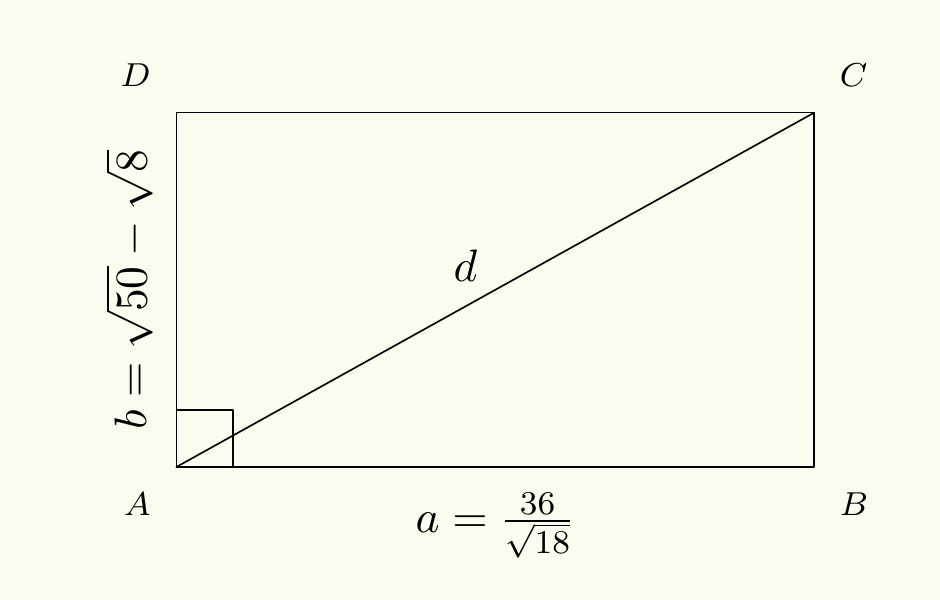
\includegraphics[max width=0.8\linewidth, max height=5cm]{../../../docs/nombres-reals/img/rectangle-diagonal-perimetre.png}
\end{center}

amb diagonal $d$. Resol sense calculadora:

\begin{enumerate}
\item Simplifica $a$ i $b$.
\item Calcula la diagonal $d$ del rectangle.
\item Calcula el perímetre $P$ i escriu-lo de la forma més senzilla possible.
\end{enumerate}

\textbf{Solució}

\begin{enumerate}
\item Simplificació de $a$ i $b$:

\[
\begin{aligned}
a &= \frac{36}{\sqrt{18}} \cdot \frac{\sqrt{18}}{\sqrt{18}} = \frac{36\sqrt{18}}{18} \\
&= 2\sqrt{18} = 2 \sqrt{3^2\cdot 2} = 6 \sqrt{2}
\end{aligned}
\]

\[
b=\sqrt{50}-\sqrt{8}
=\sqrt{5^2\cdot 2}-\sqrt{2^2\cdot 2}
=5\sqrt{2}-2\sqrt{2}
=3\sqrt{2}.
\]
\item Diagonal (teorema de Pitàgores):

\[
\begin{aligned}
d&=\sqrt{a^2+b^2} \\
&=\sqrt{\left(6\sqrt{2}\right)^2+\left(3\sqrt{2}\right)^2} \\
&=\sqrt{36\cdot 2 + 9\cdot 2} \\
&=\sqrt{90}=\sqrt{9\cdot 10}=3\sqrt{10}.
\end{aligned}
\]
\item Perímetre:

\[
P=2(a+b)=2\bigl(6\sqrt{2}+3\sqrt{2}\bigr) = 18\sqrt{2}.
\]
\end{enumerate}
\end{exemple}

\begin{nota}{Teorema de Pitàgores}
En un triangle rectangle, el quadrat de la hipotenusa és igual a la suma dels quadrats dels catets:

\[
c^2 = a^2 + b^2.
\]

Coneixent els catets $a$ i $b$, la hipotenusa s'obté amb $c = \sqrt{a^2+b^2}$. El radical $\sqrt{\phantom{a}}$ dona sempre l'arrel positiva, que és la que volem: la longitud del costat d'un triangle mai és negativa.
\end{nota}

\subsection{Taula resum}

\begin{center}
\begin{tabular}{ll}
\toprule
\textbf{Propietat} & \textbf{Expressió} \\
\midrule
Definició d'arrel & $b=\sqrt[n]{a} \iff b^n=a$ \\
Arrel com a potència & $a^{\tfrac{m}{n}} = \sqrt[n]{a^m} = \left(\sqrt[n]{a}\right)^m$ \\
Existència ($n$ parell) & $a<0 \Rightarrow$ sense arrel real; $a\ge 0 \Rightarrow \pm\sqrt[n]{a}$ \\
Existència ($n$ senar) & sempre existeix, i és única: $\sqrt[n]{a}$ \\
Simplificació/amplificació & $\sqrt[np]{a^{mp}} = \sqrt[n]{a^{m}}$ \\
Producte, mateix índex & $\sqrt[n]{a}\cdot\sqrt[n]{b} = \sqrt[n]{ab}$ \\
Quocient, mateix índex & $\dfrac{\sqrt[n]{a}}{\sqrt[n]{b}} = \sqrt[n]{\tfrac{a}{b}}$ \\
Producte/quocient, índex diferent & amplifica primer a índex $k=\mathrm{mcm}(n,m)$ \\
Arrel d'una arrel & $\sqrt[n]{\sqrt[m]{a}} = \sqrt[n\cdot m]{a}$ \\
Potència d'una arrel & $\left(\sqrt[n]{a}\right)^m = \sqrt[n]{a^m}$ \\
Racionalització (monomi) & $\dfrac{c}{\sqrt{a}} = \dfrac{c\sqrt{a}}{a}$ \\
Racionalització (binomi, conjugat) & $\dfrac{1}{a-\sqrt{b}} = \dfrac{a+\sqrt{b}}{a^2-b}$ \\
\bottomrule
\end{tabular}
\end{center}

\section{Logaritmes}

\subsection{Definició}

Imagina que et demanen quin exponent cal aplicar a una base per obtenir un cert resultat: si $a^n = b$, quant val $n$? Aquest és exactament el problema que resolen els logaritmes.

\begin{definicio}{Definició: logaritme}
Siguin $a$ i $b$ dos nombres reals amb $a>0$, $a \neq 1$ i $b>0$. El \textbf{logaritme en base $a$ de $b$} és el nombre real $n$ tal que

\[
\log_a b = n
\quad \Leftrightarrow \quad
a^n = b.
\]
\end{definicio}

\begin{nota}{Condicions de definició}
Recorda: cal $a>0$, $a\neq 1$ i $b>0$.

$\log_2 0$ no té sentit, perquè cap exponent $n$ fa $2^n=0$. Tampoc $\log_{-3} 9$: és cert que $(-3)^2=9$, però la funció $n \mapsto (-3)^n$ no està ben definida per a tot $n$ real (què seria $(-3)^{1/2}$?). Per això la base sempre ha de ser positiva.
\end{nota}

\begin{nota}{Una mica d'història}
El terme \emph{logaritme} prové del grec: \emph{logos} (raó, proporció) i \emph{arithmos} (nombre). El va encunyar \textbf{John Napier} (1550–1617), matemàtic escocès, al llibre \emph{Mirifici Logarithmorum Canonis Descriptio} (1614). El seu objectiu: convertir multiplicacions i divisions en sumes i restes, molt més ràpides de calcular a mà.
\end{nota}

Potències, arrels i logaritmes són, en el fons, la mateixa relació $a^n=b$ mirada des de tres angles diferents:

\begin{center}
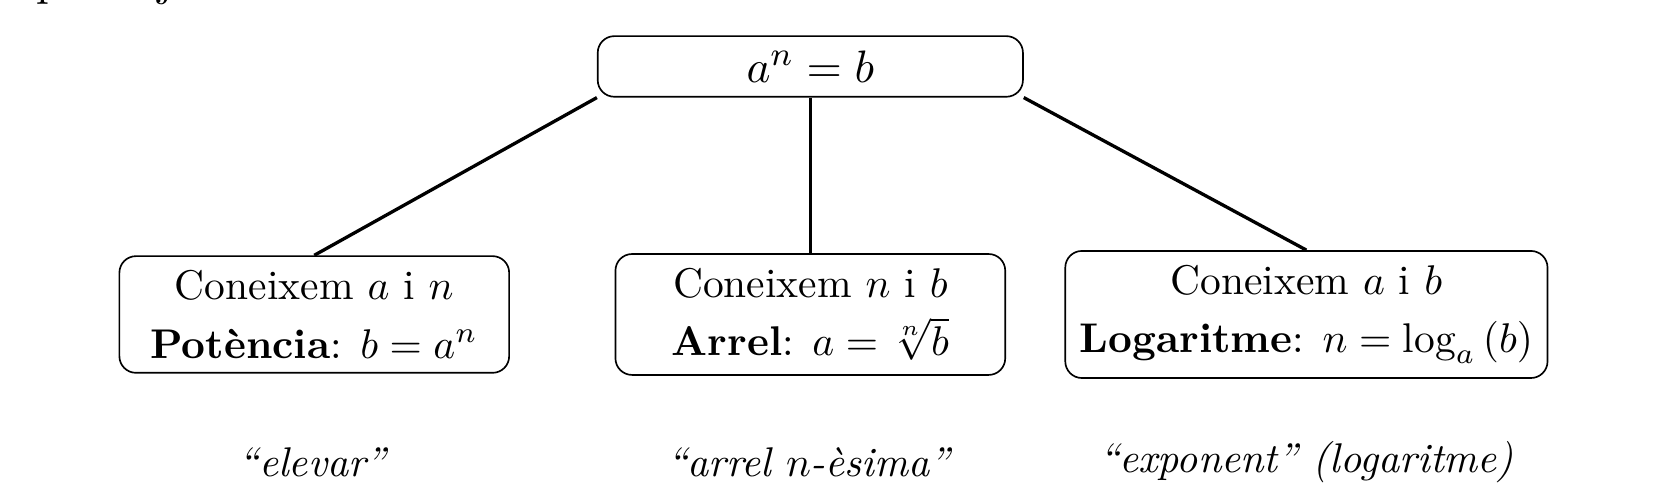
\includegraphics[max width=0.8\linewidth, max height=5cm]{../../../docs/nombres-reals/img/triangle-potencia-arrel-log.png}
\end{center}

Per això, com veurem, les propietats dels logaritmes (i de les arrels) no fan res més que traduir les propietats que ja coneixem de les potències.

\begin{exemple}{\textbf{Exemple:} Triple equivalència amb nombres concrets}
Fixa't en $2^3=8$: aquesta relació es pot escriure de tres maneres equivalents:

\[
2^3 = 8
\quad \Leftrightarrow \quad
\sqrt[3]{8}=2
\quad \Leftrightarrow \quad
\log_2 8=3.
\]
\end{exemple}

\subsubsection{Casos especials de logaritmes}

Hi ha dos casos que tenen nom i notació propis, perquè els fem servir constantment:

\begin{nota}{El nombre $e$}
El nombre $e \approx 2{,}718281828459045\ldots$ és una constant irracional amb un paper clau en matemàtiques: apareix de manera natural en límits, derivades i creixements continus. El nom \emph{logaritme neperià} és, de fet, un homenatge al mateix Napier.
\end{nota}

\begin{itemize}
\item \textbf{Logaritme decimal.} El logaritme en base $10$ s'escriu sense subíndex: $\log_{10} x = \log x$.
\item \textbf{Logaritme neperià.} El logaritme en base $e$ s'escriu $\ln x$: $\log_e x = \ln x$.
\end{itemize}

\subsection{Propietats i exemples}

Vegem ara, una a una, les propietats dels logaritmes. Totes surten directament de la definició i de les propietats que ja coneixem de les potències.

\begin{propietat}{Propietat: logaritme de $1$}
Eleva qualsevol base $a$ (amb $a>0$, $a\neq 1$) a l'exponent $0$ i sempre obtens $1$. Per això:

\[
\log_a 1=0.
\]

\emph{Per què?} Perquè l'únic $n$ real que fa $a^{n}=1$, amb $a\neq 1$, és $n=0$.
\end{propietat}

\begin{nota}{I per què no $\log_1 1$?}
Buscar $\log_1 1$ voldria dir trobar un $n$ tal que $1^n=1$... però això és cert per a \emph{qualsevol} $n$! No hi ha un exponent únic, i per això la base mai pot valer $1$.
\end{nota}

\begin{exemple}{\textbf{Exemple}}
$\log_2 1=0$, ja que $2^{0}=1$.
\end{exemple}

\begin{propietat}{Propietat: logaritme de la base}
Si la base i el número coincideixen, l'exponent que hi porta és sempre $1$:

\[
\log_a a = 1.
\]

\emph{Per què?} Perquè $a^n=a$ només es compleix per a $n=1$.
\end{propietat}

\begin{exemple}{\textbf{Exemple}}
$\log_2 2=1$, ja que $2^{1}=2$.
\end{exemple}

\begin{propietat}{Propietat: logaritme del producte}
El logaritme transforma productes en sumes — aquest és precisament el motiu pel qual Napier els va inventar! Per a $M,N>0$:

\[
\log_a (M \cdot N) \;=\; \log_a M + \log_a N.
\]

\emph{Per què?} Si $\log_a M=m$ i $\log_a N=n$, aleshores $M \cdot N = a^m \cdot a^n = a^{m+n}$.
\end{propietat}

\begin{exemple}{\textbf{Exemple}}
\[
\log_2 6
= \log_2 (2 \cdot 3)
= \log_2 2 + \log_2 3
= 1 + \log_2 3.
\]
\end{exemple}

\begin{propietat}{Propietat: logaritme del quocient}
I, de manera semblant, els quocients es converteixen en restes. Per a $M,N>0$:

\[
\log_a \tfrac{M}{N} \;=\; \log_a M - \log_a N.
\]

\emph{Per què?} Amb $M=a^m$ i $N=a^n$, tenim $\tfrac{M}{N}=a^{m-n}$.
\end{propietat}

\begin{exemple}{\textbf{Exemple}}
\[
\log_2 3
= \log_2 \tfrac{6}{2}
= \log_2 6 - \log_2 2
= \log_2 6 - 1.
\]
\end{exemple}

\begin{propietat}{Propietat: logaritme d'una potència}
L'exponent "baixa" i multiplica. Per a $M>0$ i qualsevol $n\in\mathbb{R}$:

\[
\log_a (M^n) \;=\; n \cdot \log_a M.
\]

\emph{Per què?} Si $M=a^m$, aleshores $M^n=(a^m)^n=a^{n\cdot m}$.
\end{propietat}

\begin{exemple}{\textbf{Exemple}}
Amb aquesta propietat, calcular $\log_2 32$ és immediat:

\[
\log_2 32 = \log_2 2^5 = 5 \cdot \log_2 2 = 5.
\]
\end{exemple}

\begin{propietat}{Propietat: logaritme d'una arrel}
Una arrel $n$-èsima no és més que un exponent fraccionari, així que aquesta propietat és la germana de l'anterior. Per a $M>0$ i $n\in\mathbb{N}$, $n>0$:

\[
\log_a \sqrt[n]{M} \;=\; \tfrac{1}{n} \cdot \log_a M.
\]

\emph{Per què?} Perquè $\sqrt[n]{M}=M^{1/n}$, i apliquem la propietat de la potència.
\end{propietat}

\begin{exemple}{\textbf{Exemple}}
\[
\log_2 \sqrt{8}
= \tfrac{1}{2}\,\log_2 2^3
= \tfrac{1}{2}\cdot 3
= 1{,}5.
\]
\end{exemple}

\begin{propietat}{Propietat: canvi de base}
A la calculadora només trobem $\log$ (base $10$) i $\ln$ (base $e$). Aquesta propietat ens deixa calcular un logaritme en \emph{qualsevol} base a partir d'aquests. Amb $a,b,M>0$, $a\neq 1$, $b\neq 1$:

\[
\log_a M = \frac{\log_b M}{\log_b a}.
\]

\emph{Per què?} Si $n=\log_a M$, aleshores $a^n=M$. Prenent $\log_b$ a banda i banda i aplicant la propietat de la potència, $n\cdot\log_b a=\log_b M$, d'on surt la fórmula.
\end{propietat}

\begin{exemple}{\textbf{Exemple}}
\[
\log_2 100 = \frac{\log 100}{\log 2} = \frac{2}{\log 2} = \frac{\ln 100}{\ln 2}.
\]
\end{exemple}

\subsection{Taula resum}

Per repassar d'un cop d'ull:

\begin{center}
\begin{tabular}{ll}
\toprule
\textbf{Propietat} & \textbf{Fórmula} \\
\midrule
Logaritme de $1$ & $\log_a 1 = 0$ \\
Logaritme de la base & $\log_a a = 1$ \\
Producte & $\log_a (M\cdot N) = \log_a M + \log_a N$ \\
Quocient & $\log_a \dfrac{M}{N} = \log_a M - \log_a N$ \\
Potència & $\log_a (M^n) = n\log_a M$ \\
Arrel & $\log_a \sqrt[n]{M} = \dfrac{1}{n}\log_a M$ \\
Canvi de base & $\log_a M = \dfrac{\log_b M}{\log_b a}$ \\
Logaritme decimal & $\log_{10} x = \log x$ \\
Logaritme neperià & $\log_e x = \ln x$ \\
\bottomrule
\end{tabular}
\end{center}

\subsection{Exemples d'aplicació}

Acabem amb dos exemples reals on els logaritmes apareixen de manera natural: l'interès compost i l'equació de Hill en farmacologia.

\begin{exemple}{\textbf{Exemple:} Interès compost}
Quan un capital $C_0$ genera un interès compost del $i\%$ anual, al cap de $t$ anys tenim

\[
C_f = C_0 \left( 1 + \tfrac{i}{100}\right)^t.
\]

Suposem $C_0=7.000$ € a un $2{,}5\%$ anual. Quants anys calen, aproximadament, per arribar a $7.354$ €?

\[
7354 = 7000 \cdot 1{,}025^t
\;\Rightarrow\;
1{,}025^t = \frac{7354}{7000} \approx 1{,}050571.
\]

Apliquem la definició de logaritme i, per poder-lo calcular amb la calculadora, canviem a base neperiana:

\[
t = \log_{1{,}025} 1{,}050571
= \frac{\ln 1{,}050571}{\ln 1{,}025}
\approx \frac{0{,}049316}{0{,}024692}
\approx 1{,}998.
\]

És a dir, uns \textbf{$2$ anys}.
\end{exemple}

\begin{exemple}{\textbf{Exemple:} Equació de Hill}
En farmacologia, l'\textbf{equació de Hill} relaciona la concentració d'un fàrmac amb la resposta biològica que provoca:

\[
E = E_{max} \cdot \frac{D^n}{K_D^n+D^n},
\]

on $E_{max}$ és l'efecte màxim, $K_D$ la concentració que dona la meitat de l'efecte màxim, i $n$ (el coeficient de Hill) el que volem trobar.

Dades: $E_{max}=90\%$, $K_D=60$, i $E=80\%$ per a $D=90$. Substituint i simplificant:

\[
80 = 90 \cdot \frac{90^n}{60^n+90^n}
\;\Rightarrow\;
8\cdot 60^n = 90^n
\;\Rightarrow\;
\Bigl(\tfrac{3}{2}\Bigr)^n = 8
\]

(dividint tot entre $60^n$ i simplificant $\tfrac{90}{60}=\tfrac32$).

Ara ja és una definició de logaritme directa, amb canvi de base:

\[
n = \log_{3/2} 8
= \frac{\ln 8}{\ln \frac{3}{2}}
\;\simeq\; 5{,}13.
\]
\end{exemple}

\section{Nota històrica}

Per què costa tant acceptar que hi ha nombres que no es poden escriure com una fracció? La història dels nombres reals és, en el fons, la història d'aquesta resistència.

Primer van aparèixer els \textbf{naturals}, per comptar. Després els \textbf{enters}, per representar deutes i pèrdues. I més tard els \textbf{racionals}, quan va caldre mesurar parts d'un tot: longituds, àrees...

Fixa't en aquest fet, ocorregut a l'\textbf{Antiga Grècia}: la diagonal d'un quadrat de costat $1$ mesura $\sqrt{2}$, i aquest nombre no es pot escriure com una fracció. El descobriment va trasbalsar els pitagòrics, convençuts que tot s'explicava amb racionals. Així van néixer els \textbf{irracionals}.

Durant segles se'ls va mirar amb recel. Calgué l'àlgebra i la geometria del món \textbf{àrabo-islàmic medieval} i del \textbf{Renaixement europeu} perquè guanyessin legitimitat.

Al segle XVII, amb el \textbf{càlcul diferencial i integral} de Newton i Leibniz, es va fer evident que calia una base més sòlida. Però no va ser fins als segles XVIII i XIX que \textbf{Dedekind} i \textbf{Cantor} (amb la teoria de conjunts) en van donar una definició rigorosa.

Gràcies a això, avui podem parlar amb precisió de continuïtat, límits i funcions: tot l'edifici de les matemàtiques modernes.

Els \textbf{nombres reals} hi són, arreu: descriuen longituds, temps, temperatures, velocitats... Formen un conjunt infinit i no numerable, però la seva utilitat és fora de dubte.

\end{document}
